\documentclass[11pt]{article}
\usepackage[margin=1in]{geometry}
\usepackage{amsmath,amssymb,amsthm,mathtools,bm}
\usepackage{graphicx,booktabs,array,enumitem,xcolor}
\usepackage[numbers,sort&compress]{natbib}
\usepackage[colorlinks=true,linkcolor=blue!50!black,citecolor=blue!50!black,urlcolor=blue!50!black]{hyperref}
\usepackage[nameinlink,capitalise]{cleveref}

\newtheorem{theorem}{Theorem}
\newtheorem{lemma}[theorem]{Lemma}
\newtheorem{proposition}[theorem]{Proposition}
\newtheorem{corollary}[theorem]{Corollary}
\theoremstyle{definition}
\newtheorem{definition}[theorem]{Definition}
\newtheorem{assumption}{Assumption}
\theoremstyle{remark}
\newtheorem{remark}[theorem]{Remark}
\newtheorem{example}[theorem]{Example}

\crefname{assumption}{Assumption}{Assumptions}

\newcommand{\R}{\mathbb{R}}
\newcommand{\E}{\mathbb{E}}
\newcommand{\tr}{\operatorname{tr}}
\newcommand{\diag}{\operatorname{diag}}
\newcommand{\Var}{\operatorname{Var}}
\newcommand{\Cov}{\operatorname{Cov}}
\newcommand{\bits}{\operatorname{bits}}
\newcommand{\Em}{\mathcal{E}}         % the energy metric matrix
\newcommand{\Ht}{\tilde{H}}
\newcommand{\At}{\tilde{A}}
\newcommand{\Jt}{\mathcal{J}}
\newcommand{\Rt}{\mathcal{R}}
\newcommand{\ip}[2]{\langle #1,\,#2\rangle}
\newcommand{\codeus}{\textunderscore\allowbreak}
\newcommand{\code}[1]{{\ttfamily\let\_\codeus\hyphenchar\font=-1 #1}}
\setlength{\emergencystretch}{3em}
\newcommand{\checked}[1]{\par\smallskip\noindent\textit{Numerical check.} #1\par}
\newcommand{\phys}[1]{\par\smallskip\noindent\textit{What this means physically.} #1\par}

\title{Energy-based whitening for information-theoretic analysis of mechanisms:\\
theory, relation to the literature, and practice}
\author{Companion note to \emph{Quantifying Mechanical Intelligence in Legged Robots}\\
\emph{with Information Theory} (arXiv:2609.19588)}
\date{}

\begin{document}
\maketitle

\begin{abstract}
The paper whitens the mechanical state with the energy metric $\Em = \diag(K,H)$, setting
$x = \Em^{1/2}x_q$, and then adds isotropic noise (its Eq.~(9)). It gives this step two
sentences and five citations. This note supplies the missing theory.
\begin{itemize}[nosep]
  \item Mutual information does not change under invertible maps, so whitening has content
        \emph{only} through the noise model it implies. That model is Gaussian noise of
        covariance $\sigma^2\Em^{-1}$ on the physical state: the maximum-entropy noise at
        fixed mean energy, which is also the Gibbs/equipartition fluctuation law.
  \item From that one fact the note proves, in elementary steps:
  \begin{itemize}[nosep]
    \item exact invariance of every bit count under linear changes of generalized
          coordinates (units, gearing, relative coordinates);
    \item a port-Hamiltonian structure of the whitened dynamics, whose singular values are
          the natural frequencies;
    \item a general \emph{constraint-limit} theorem: an energy-whitened stiff
          series-elastic actuator (SEA) converges, bit for bit, to the rigid transmission;
    \item the exact size of the artifact that per-coordinate noise produces instead
          (8.47 bits on the paper's model);
    \item the low- and high-SNR asymptotics, which explain why the design comparison
          does not depend on the noise scale;
    \item a consistent noise model for Shapley attribution, which shows that redundant
          \emph{positions} split credit equally but redundant \emph{velocities} split it
          by inertia;
    \item a closed form for the Zahedi--Ay morphological-computation metric that explains
          the tension the paper reports.
  \end{itemize}
  \item Related problems:
  \begin{itemize}[nosep]
    \item energy whitening makes information counts for continuum (finite-element)
          bodies independent of the mesh, whereas per-node noise grows without bound;
    \item it identifies exactly when a floating base's singular metric loses information.
  \end{itemize}
\end{itemize}
Part~II asks whether energy is the \emph{right} choice.
\begin{itemize}[nosep]
  \item Maximum entropy fixes the noise's shape only once energy is chosen. The choice
        itself is justified by a uniqueness theorem: energy is the only noise metric that
        is coordinate-free, local, free of outside scales, time-symmetric, and invariant
        under free motion.
  \item The last property is equivalent to ``free motion never creates information.''
        Under energy noise, information changes only through work and dissipation.
  \item The alternatives are compared: per-coordinate, kinetic, frequency-weighted
        (including the quantum-like action weighting), and data-driven.
  \item A thermodynamically consistent \emph{Langevin body}, with noise injected through
        its dampers, shows that with the full state observed every design is capped at the
        same contact-damping limit. Morphology matters by \emph{routing} information to
        the sensors: the rigid transmission delivers 99.9\% of the limit to its motor
        encoder, and the SEA climbs from 6\% to 99.5\% with stiffness.
\end{itemize}
Every claim is checked numerically on the repository's own models.
\end{abstract}

\tableofcontents

%=========================================================================================
\section{The idea in plain language}
\label{sec:plain}

This section explains the whole idea without proofs. The rest of the note makes each
sentence precise.

\paragraph{A deterministic mechanism carries infinite information.} The paper asks how much
the leg's motion tells us about the force that pushed it. The leg obeys deterministic
equations. If we knew them exactly and could read the state with perfect precision, we
could run them backward and recover the force exactly. Recovering a real number exactly
corresponds to infinitely many bits. So, strictly, every mechanism carries infinite
information about the force, and comparing two designs would give ``$\infty$ vs
$\infty$.'' To get a finite answer we must say how precisely the state can be known; that
is, we must add noise. The noise is not a nuisance on top of the analysis. It \emph{is}
the definition of resolution, and the answer depends on it.

\paragraph{Relabeling changes nothing.} If you transform the observed quantity in a way
that can be undone, the information stays the same. This covers converting meters to
millimeters, rotating axes, or multiplying the state by any invertible matrix. Anything
learnable from the original is learnable from the transformed version by undoing the
transformation first, and vice versa.

Whitening, $x=\Em^{1/2}x_q$, is such a transformation, so on its own it changes nothing.
It matters only because of the order of operations: first transform, then add noise of the
same size in every direction. Adding equal noise \emph{after} the transformation is the
same as adding a particular, unequal noise \emph{before} it. So ``energy whitening'' is
really a statement about what the noise on the physical state looks like.

\paragraph{What the noise looks like.} Take a mass $m$ on a spring of stiffness $k$, with
position $q$ and velocity $\dot q$. Whitening gives $x=(\sqrt k\,q,\sqrt m\,\dot q)$. Its
squared length $kq^2+m\dot q^2$ is twice the stored energy, and every component is
measured in $\sqrt{\mathrm J}$. Adding noise of standard deviation $\sigma$ to both
components means, back in physical units:
\begin{itemize}[nosep]
  \item position noise of standard deviation $\sigma/\sqrt k$;
  \item velocity noise of standard deviation $\sigma/\sqrt m$.
\end{itemize}
So stiff springs make position precise, and heavy masses make velocity precise. The reason
is that both blurs carry \emph{the same energy}, $\frac12\sigma^2$. The rule being imposed
is: \emph{two states that differ by less than a fixed amount of energy cannot be told
apart.}

Geometrically, the noise has the constant-energy ellipses as its contour lines
(\cref{fig:ellipse}a). The alternative, ``add the same noise to each coordinate,'' asserts
that an error of $10^{-4}$\,rad in an angle and $10^{-4}$\,rad/s in a velocity are equally
hard to detect (\cref{fig:ellipse}b). The two quantities do not even share units, and the
assertion changes when the units do.

\begin{figure}[t]\centering
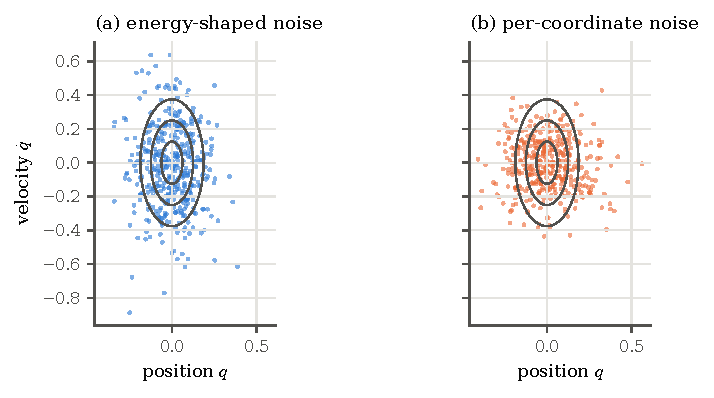
\includegraphics[width=0.82\linewidth]{figures/ellipse.pdf}
\caption{A mass on a spring ($k=4$, $m=1$, illustrative units). Grey curves are
constant-energy ellipses. (a) Energy-shaped noise has the same ellipses as its contours:
every perturbation of equal energy is equally likely. (b) Per-coordinate noise is round in
whatever units the coordinates happen to use.}
\label{fig:ellipse}
\end{figure}

\paragraph{Why this noise: maximum entropy.} Suppose the only thing we are willing to
commit to is the noise's average energy. Choosing a distribution means making assumptions:
a sharply peaked distribution claims to know a lot, and a lopsided one claims some
directions matter more. The standard measure of how few assumptions a distribution makes
is its \emph{entropy}. Jaynes' \emph{principle of maximum entropy} says: among all
distributions consistent with what you know, choose the one with the largest entropy.

Among all noise laws with a given average energy, the largest-entropy one is
$p\propto\exp(-\text{energy}/T)$. For quadratic energy this is a Gaussian with covariance
$T\,\Em^{-1}$, which is exactly the noise above, with $T=\sigma^2$. In whitened coordinates
the constraint is simply ``average squared length is fixed,'' which treats every direction
alike. The most even way to spread a fixed average squared length is the round Gaussian.

\paragraph{Gibbs and equipartition.} The formula $p\propto\exp(-\text{energy}/T)$ is the
Gibbs (Boltzmann) distribution: the law of a system in equilibrium with a heat bath. It
implies \emph{equipartition}: every quadratic term in the energy holds $\frac12k_BT$ on
average. For the mass on a spring, $\langle q^2\rangle=k_BT/k$ and $\langle\dot
q^2\rangle=k_BT/m$, exactly the variances above. So the paper's noise blurs the body as if
it were jiggling thermally at temperature $\sigma^2$.

That temperature is a \emph{resolution} written in energy units, not real heat: the
repository's $\sigma^2=10^{-4}$\,J is about $10^{16}$ times room-temperature $k_BT$. Only
the \emph{shape} of the noise is fixed by physics. Its \emph{size} mostly sets the zero of
the bit scale.

\paragraph{Why it solves the paper's problem.} The SEA has an extra coordinate, the motor
angle. As the spring stiffens it moves in lockstep with the joint angle.
\begin{itemize}[nosep]
  \item \emph{With per-coordinate noise}, the motor angle becomes a second, independently
        noisy reading of the same signal. That is worth about half a bit per force mode,
        8.47 bits here, so a stiff SEA appears ``smarter'' than the rigid leg it has
        physically become.
  \item \emph{With energy noise}, this cannot happen. A direction of motion earns
        information only through the energy it stores, so relabeling or duplicating
        coordinates never creates bits.
\end{itemize}

\paragraph{Is it the best choice?} Part~II (\cref{sec:right,sec:alternatives,sec:langevin,sec:capture})
asks this directly.
\begin{itemize}[nosep]
  \item Maximum entropy justifies the noise's \emph{shape} once energy is chosen, not the
        choice of energy itself.
  \item That choice is justified separately: energy is the only noise metric with five
        physical properties, the decisive one being that free motion can never create
        information.
  \item A noise model is not yet a measure of computation. A thermodynamically consistent
        ``Langevin body'' shows what morphology can and cannot do.
\end{itemize}

%=========================================================================================
\section{Setup, notation, and what is being asked}
\label{sec:setup}

\paragraph{The mechanism.} A linear(ized) mechanism with $n$ generalized coordinates
$q\in\R^n$ obeys
\begin{equation}\label{eq:eom}
  H\ddot q + D\dot q + Kq = J^\top f(t),
\end{equation}
where:
\begin{itemize}[nosep]
  \item $H=H^\top\succ0$ is the mass matrix;
  \item $K=K^\top\succeq0$ is the stiffness, including the ground spring $J^\top k_iJ$;
  \item $D=D^\top\succeq0$ is the damping;
  \item $J$ maps generalized velocity to foot velocity, so $f$ enters through $J^\top$.
\end{itemize}
The state is $x_q=(q,\dot q)\in\R^{2n}$, and \eqref{eq:eom} reads
$\dot x_q = Ax_q + B f$ with
\begin{equation}\label{eq:AB}
  A=\begin{bmatrix}0&I\\-H^{-1}K&-H^{-1}D\end{bmatrix},\qquad
  B=\begin{bmatrix}0\\H^{-1}J^\top\end{bmatrix}.
\end{equation}

\paragraph{The energy metric.} Following the paper's Eq.~(9), define
\begin{equation}\label{eq:metric}
  \Em=\begin{bmatrix}K&0\\0&H\end{bmatrix},\qquad x=\Em^{1/2}x_q .
\end{equation}
Here $\Em^{1/2}$ is the symmetric positive semidefinite square root
(\code{mechinfo.mechanics.sym\_sqrt}). Because $\Em$ is block diagonal, $\Em^{1/2} =
\diag(K^{1/2},H^{1/2})$. We write $\Em$ rather than the paper's $E$ so that $\E$ can denote
expectation. When $K\succ0$ we say the metric is \emph{nondegenerate}.

\paragraph{The channel.} The unknown force over a window $[0,T]$ is expanded in $d$ basis
functions, $f(t)=\sum_{j=1}^d w_j\varphi_j(t)$ with $w\sim\mathcal N(0,\sigma_w^2I_d)$
(the paper's Eq.~(8)). The state is sampled at $t_k=k/f_s$, $k=0,\dots,N_t-1$. A readout
matrix $C$ is applied, and i.i.d.\ noise $n_k\sim\mathcal N(0,\sigma^2 I)$ is added:
\begin{equation}\label{eq:channel}
  y_k = C x_q(t_k) + n_k,\qquad y = Mw + n .
\end{equation}
Here $M$ stacks the responses: column $j$ of $M$ is the sampled readout of the response to
$\varphi_j$. Write $X_k\in\R^{2n\times d}$ for the matrix whose column $j$ is the state at
$t_k$ under input $\varphi_j$, so that $M=[CX_0;\dots;CX_{N_t-1}]$. The energy readout is
$C=\Em^{1/2}$ with noise scale $\sigma$ in $\sqrt{\mathrm J}$
(\code{passive\_info.information.SIGMA\_ENERGY}).

\begin{lemma}[Gaussian channel]\label{lem:gauss}
For \eqref{eq:channel},
\[
  I(w;y)=\tfrac12\log\det\!\big(I_d+\gamma M^\top M\big),\qquad \gamma=\sigma_w^2/\sigma^2 ,
\]
and the right-hand side depends on $C$ only through the $d\times d$ \emph{Gram matrix}
\begin{equation}\label{eq:gram}
  G \;=\; \gamma M^\top M \;=\; \gamma\sum_{k} X_k^\top\,(C^\top C)\,X_k .
\end{equation}
\end{lemma}
\begin{proof}
\begin{enumerate}[nosep]
  \item Given $w$, $y$ is Gaussian with covariance $\sigma^2I$, so
        $h(y\mid w)=\frac12\log\det(2\pi e\,\sigma^2 I)$.
  \item Unconditionally, $y$ is Gaussian with covariance $\sigma^2I+\sigma_w^2MM^\top$, so
        $h(y)=\frac12\log\det(2\pi e(\sigma^2I+\sigma_w^2MM^\top))$.
  \item Subtracting, $I(w;y)=h(y)-h(y\mid w)=\frac12\log\det(I+\gamma MM^\top)$.
  \item Sylvester's identity, $\det(I+PQ)=\det(I+QP)$, replaces $MM^\top$ by $M^\top M$.
  \item Finally, $M^\top M=\sum_k (CX_k)^\top(CX_k)=\sum_kX_k^\top C^\top CX_k$.
\end{enumerate}
\end{proof}

Throughout, ``bits'' means $\bits(G)=\tfrac12\log_2\det(I+G)$
(\code{mechinfo.mechanics.bits\_from\_gram}). The paper's Eq.~(3) writes the same formula
with $K$ for the input covariance. That clashes with the stiffness $K$ of Eq.~(5); a
revision could use $\Sigma_w$.

\paragraph{The question.} \Cref{lem:gauss} already shows that the readout enters only
through $C^\top C$. Whitening by $\Em^{1/2}$ therefore amounts to declaring
$C^\top C=\Em$. The rest of this note asks:
\begin{enumerate}[nosep]
  \item why this is the right declaration;
  \item what it buys, mathematically and for the paper's problems;
  \item where it fails.
\end{enumerate}

\paragraph{Models used for the checks.} The checks use:
\begin{itemize}[nosep]
  \item the paper's clamped one-leg model, both the rigid (proprioceptive) transmission
        $q=\theta$ and the SEA $q=(\theta_j,\theta_m)$, with the parameters of Section~III
        (taken from \citet{wensing2017proprioceptive});
  \item band $B_w=100$\,Hz unless stated ($d=17$ modes), window $T=85$\,ms, and
        $f_s=4$\,kHz.
\end{itemize}
All numbers come from \code{docs/whitening/checks.py}. Pytest versions are in
\code{tests/test\_energy\_whitening.py}.

%=========================================================================================
\section{What whitening is, and what it is not}
\label{sec:what}

\begin{lemma}[Only the noise model matters]\label{lem:noise}
Let $S$ be an invertible matrix and let $X$ be any random vector.
\begin{enumerate}[label=(\alph*)]
  \item $I(w;SX)=I(w;X)$.
  \item Without noise, the information is infinite: if $M\neq0$, then $I(w;Mw)=\infty$.
  \item $I(w;\,\Em^{1/2}x_q+n)=I(w;\,x_q+\Em^{-1/2}n)$ when $\Em\succ0$. Hence isotropic
        noise on the whitened state is \emph{the same channel} as noise
        $\nu=\Em^{-1/2}n\sim\mathcal N(0,\sigma^2\Em^{-1})$ added to the physical state.
\end{enumerate}
\end{lemma}
\begin{proof}
(a) The map $X\mapsto SX$ is a bijection, with inverse $S^{-1}$. By the data-processing
inequality, $I(w;SX)\le I(w;X)$ because $SX$ is computed from $X$. Equally,
$I(w;X)\le I(w;SX)$ because $X=S^{-1}(SX)$ is computed from $SX$. So the two are equal.

(b) For any $\varepsilon>0$, the vector $Mw+\varepsilon n$ is computed from $Mw$ and an
independent $n$. Data processing therefore gives $I(w;Mw)\ge I(w;Mw+\varepsilon n)$. By
\cref{lem:gauss} the right-hand side is
$\frac12\log\det(I+\sigma_w^2\varepsilon^{-2}M^\top M)$. At least one eigenvalue of
$M^\top M$ is positive, so this tends to $\infty$ as $\varepsilon\to0$.

(c) Apply (a) with $S=\Em^{-1/2}$ to the observation $\Em^{1/2}x_q+n$. That gives
$x_q+\Em^{-1/2}n$. The covariance of $\Em^{-1/2}n$ is
$\Em^{-1/2}(\sigma^2I)\Em^{-1/2}=\sigma^2\Em^{-1}$.
\end{proof}

\phys{The trajectory of a deterministic mechanism determines the force exactly. Without a
declared resolution the bit count is infinite, and that is a property of the analysis,
not of the body (\code{sim\_info.\_observe} makes the same point in a comment). Whitening
is \emph{not} a preprocessing step that changes the information. Its entire content is the
statement \emph{``the body's state is known to within a Gaussian blur of covariance
$\sigma^2\Em^{-1}$.''} In communication-theory terms, $\Em^{1/2}$ is the
\emph{noise-whitening filter} for that colored noise. Applying it before the
isotropic-noise formula is the standard way to compute capacity with colored noise
\citep{cover2006elements}.}

\begin{lemma}[Energy identity]\label{lem:energy}
$|x|^2=x_q^\top\Em x_q=q^\top Kq+\dot q^\top H\dot q=2(V+T_{\rm kin})$, which is twice the
stored mechanical energy. Every component of $x$ therefore has units of $\sqrt{\mathrm J}$.
\end{lemma}
\begin{proof}
$|x|^2=x_q^\top\Em^{1/2}\Em^{1/2}x_q=x_q^\top\Em x_q$. Expanding the block-diagonal form
gives the rest.
\end{proof}

\begin{lemma}[Every square root gives the same bits]\label{lem:roots}
Let $C$ be any readout with $C^\top C=\Em$. Examples are the symmetric root
$\Em^{1/2}$, the upper Cholesky factor, and any $U\Em^{1/2}$ with $U^\top U=I$. Then every
such $C$ produces the same Gram matrix \eqref{eq:gram}, and so the same bits.
Conversely, if $C$ is square and invertible with $C^\top C=\Em$, then $C=U\Em^{1/2}$ for an
orthogonal $U$.
\end{lemma}
\begin{proof}
The first claim is immediate from \eqref{eq:gram}, which contains $C$ only as $C^\top C$.

For the converse, put $U=C\Em^{-1/2}$. Then
$U^\top U=\Em^{-1/2}C^\top C\Em^{-1/2}=\Em^{-1/2}\Em\,\Em^{-1/2}=I$, so $U$ is orthogonal.
\end{proof}

\begin{remark}[Relation to statistical whitening]
\Cref{lem:roots} is the mechanical version of the rotational freedom of whitening noted
by \citet[Eq.~(4)]{kessy2018optimal}: every whitening matrix has the form
$W=Q_1\Sigma^{-1/2}$ with $Q_1$ orthogonal. Among these, the symmetric
(ZCA--Mahalanobis) choice $W=\Sigma^{-1/2}$ (their Eq.~(8)) is the unique one that
minimizes $\E|z-x|^2$ (their Eqs.~(13)--(14)). With $\Sigma=\sigma^2\Em^{-1}$ that whitener
is $\Em^{1/2}/\sigma$.

The repository's choice of the symmetric root is therefore the one that keeps whitened
coordinates as close as possible to the original ones. Bits do not depend on that choice.
\code{embodied.sim\_profile\_bits} uses $\sum_kX_k^\top\Em X_k$ directly, and
\code{sim\_info} uses $\Em^{1/2}$; by \cref{lem:roots} the two agree.
\end{remark}

\checked{The symmetric root, the Cholesky factor, the direct Gram, and physical noise
$\sigma^2\Em^{-1}$ (block-diagonal over time) all give 71.77253 bits for the SEA at
$k_s=10^4$. They agree to $10^{-13}$ (\code{check\_square\_roots},
\code{check\_noise\_equivalence}).}

%=========================================================================================
\section{Invariance and the noise law}
\label{sec:invariance}

\subsection{Exact invariance under linear changes of coordinates}

Suppose the same mechanism is described in new coordinates $\tilde q$, related by
$q=T\tilde q$ with $T$ constant and invertible. Examples: radians to degrees; joint and
motor angles to joint angle and spring deflection $\delta=\theta_j-\theta_m$; a motor
angle measured before or after a gear.

\begin{theorem}[Coordinate invariance]\label{thm:invariance}
Under $q=T\tilde q$, the energy-whitened Gram matrix, and hence every bit count computed
from it, is \emph{identical} in the two descriptions. This includes chain-rule band
decompositions, which are functions of sub-blocks of $G$.

By contrast, for per-coordinate noise with a fixed diagonal weight $\Lambda$ (i.e.
$C^\top C=\Lambda$ in both descriptions), the Gram changes from $\sum_kX_k^\top\Lambda X_k$
to $\sum_kX_k^\top\mathcal T^{-\top}\Lambda\mathcal T^{-1}X_k$, where
$\mathcal T=\diag(T,T)$. This differs unless $\mathcal T$ preserves $\Lambda$.
\end{theorem}
\begin{proof}
\emph{Step 1: how the matrices transform.} Kinetic energy, potential energy, Rayleigh
dissipation and virtual work are scalars, so they must take the same value in both
descriptions:
\begin{itemize}[nosep]
  \item $\tfrac12\dot q^\top H\dot q=\tfrac12\dot{\tilde q}^\top(T^\top HT)\dot{\tilde q}$;
  \item $\tfrac12q^\top Kq=\tfrac12\tilde q^\top(T^\top KT)\tilde q$;
  \item $\tfrac12\dot q^\top D\dot q=\tfrac12\dot{\tilde q}^\top(T^\top DT)\dot{\tilde q}$;
  \item $f\cdot J\delta q=f\cdot (JT)\delta\tilde q$.
\end{itemize}
So $\tilde H=T^\top HT$, $\tilde K=T^\top KT$, $\tilde D=T^\top DT$ and $\tilde J=JT$.
Equivalently, substitute $q=T\tilde q$ into \eqref{eq:eom} and multiply on the left by
$T^\top$.

\emph{Step 2: same trajectories.} If $q(t)$ solves \eqref{eq:eom} from rest, then
$\tilde q(t)=T^{-1}q(t)$ solves the transformed equation from rest. Solutions of linear
ODEs are unique, so this is \emph{the} transformed trajectory. Hence
$\tilde X_k=\mathcal T^{-1}X_k$ for every $k$.

\emph{Step 3: same Gram.} The new metric is
$\tilde\Em=\diag(\tilde K,\tilde H)=\mathcal T^\top\Em\,\mathcal T$. Therefore
\[
  \sum_k\tilde X_k^\top\tilde\Em\tilde X_k
  =\sum_k X_k^\top\mathcal T^{-\top}\mathcal T^\top\Em\,\mathcal T\mathcal T^{-1}X_k
  =\sum_kX_k^\top\Em X_k .
\]
The same computation with $\Lambda$ in place of $\tilde\Em$ gives the second claim.
\end{proof}

\phys{The energy inner product $\ip{x_q}{x_q'}_\Em=x_q^\top\Em x_q'$ between two states is a
physical quantity: (twice) a cross-energy. It does not care what you called the
coordinates. A per-coordinate noise budget asserts that ``one unit'' of motion in each
coordinate is equally distinguishable, and that assertion changes when the coordinates do.}

\begin{example}[Radians versus degrees]\label{ex:degrees}
Relabel both SEA angles in degrees ($T=\frac{\pi}{180}I$) and keep a per-coordinate noise
of fixed numerical size. Then $\mathcal T^{-\top}\Lambda\mathcal T^{-1}=c\Lambda$ with
$c=(180/\pi)^2\approx3283$, so the Gram is multiplied by $c$.

If all $d=17$ modes are well excited, the high-SNR formula of \cref{prop:snr} predicts a
gain of
$\frac12\cdot17\cdot\log_2c=99.29$ bits. The exact gain is
$\frac12\sum_i\log_2\frac{1+c\lambda_i}{1+\lambda_i}=99.258$ bits, and the code returns
$180.62-81.37=99.258$ bits. The energy-whitened count is 71.77253 bits in both cases
(\cref{fig:invariance}).
\end{example}

\begin{figure}[t]\centering
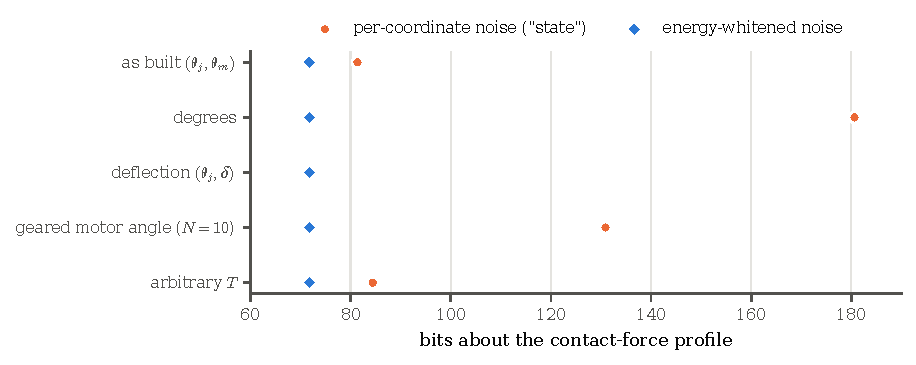
\includegraphics[width=0.92\linewidth]{figures/invariance.pdf}
\caption{The same SEA ($k_s=10^4$) described in five sets of generalized coordinates.
Energy whitening gives 71.77253 bits every time; the spread is $3\times10^{-14}$. A
per-coordinate noise budget gives anything from 71.6 to 180.6 bits
(\code{check\_invariance}).}
\label{fig:invariance}
\end{figure}

\begin{remark}[Scope: nonlinear coordinates, and what Shapley values inherit]\label{rem:scope}
\begin{enumerate}[nosep]
  \item \emph{Nonlinear reparametrizations.} For $q=\phi(\tilde q)$, the kinetic energy
        transforms exactly: $\tilde H(\tilde q)=D\phi^\top H(\phi(\tilde q))D\phi$, because
        $H(q)$ is a Riemannian metric. The stiffness Hessian transforms tensorially only
        at an equilibrium, where $\nabla V=0$; elsewhere a term
        $\sum_i\partial_iV\,\nabla^2\phi_i$ appears.
  \item \emph{Consequence for the simulator.} The MuJoCo leg freezes $\Em$ at the stance
        pose (\code{embodied.\_sim\_metric}). That is exact to first order in the
        deflection. A natural refinement is to whiten velocities with $H(q(t))$ along the
        trajectory. This is exactly invariant under any smooth reparametrization and costs
        one \code{mj\_fullM} call per sample.
  \item \emph{Shapley values.} The \emph{total} bits are coordinate-free, but a Shapley
        attribution \emph{over coordinates} is not: its players are the coordinates.
        Attributing over $(\theta_j,\delta)$ gives different shares from attributing over
        $(\theta_j,\theta_m)$. Shares are meaningful when the players are physically
        meaningful (sensor sites, modes); see \cref{sec:shapley}.
\end{enumerate}
\end{remark}

\begin{remark}[Relation to geometric identification]
\citet{lee2020geometric} (paper [24]) pursue the same goal in a different space. As we
understand it from secondary sources, they replace Euclidean distances between inertial
parameters by a coordinate-invariant Riemannian metric on positive-definite pseudo-inertia
matrices. That makes identification independent of the body frame.

Energy whitening does the analogous thing on the \emph{state} space. A physically defined
positive-definite form ($\Em$, rather than the pseudo-inertia) fixes the geometry, so that
results do not depend on the coordinates (\cref{thm:invariance}). The analogy is
conceptual: the two metrics live on different spaces and serve different purposes.
\end{remark}

\subsection{Why this noise: maximum entropy at fixed energy}

\begin{theorem}[Maximum entropy]\label{thm:maxent}
Let $\Em\succ0$ be $m\times m$ and $\sigma>0$. Among all probability densities $p$ on
$\R^m$ with mean energy budget $\E_p[\nu^\top\Em\nu]=m\sigma^2$, the differential
entropy is uniquely maximized by $g=\mathcal N(0,\sigma^2\Em^{-1})$.
\end{theorem}
\begin{proof}
\emph{Step 1: the log-density of $g$.}
\[
  \log g(\nu)=-\tfrac12\log\det(2\pi\sigma^2\Em^{-1})-\frac{\nu^\top\Em\nu}{2\sigma^2}.
\]

\emph{Step 2: average it under any admissible $p$.} The constraint fixes
$\E_p[\nu^\top\Em\nu]=m\sigma^2$, so
\[
  -\E_p[\log g]=\tfrac12\log\det(2\pi\sigma^2\Em^{-1})+\tfrac m2 .
\]
This number does not depend on which admissible $p$ we chose. In particular it equals
$-\E_g[\log g]=h(g)$, since $g$ is itself admissible:
$\E_g[\nu^\top\Em\nu]=\tr(\Em\,\sigma^2\Em^{-1})=m\sigma^2$.

\emph{Step 3: Gibbs' inequality.}
\[
  0\le \mathrm{KL}(p\,\|\,g)=\E_p[\log p]-\E_p[\log g]=-h(p)+h(g).
\]
So $h(p)\le h(g)$, with equality if and only if $p=g$ almost everywhere.
\end{proof}

\phys{If the only thing we are willing to assert about the body's resolution is
\emph{how much energy} an indistinguishable perturbation carries, the least committal
noise law \citep[Sec.~2]{jaynes1957information} is $\mathcal N(0,\sigma^2\Em^{-1})$.
In whitened coordinates this is isotropic noise, which is exactly what the paper adds.

Jaynes treats the discrete case (his Eqs.~(2-4) and (2-10), with the Boltzmann
distribution in Sec.~3), and his footnote~6 sets the continuous case aside. The
continuous argument above is the standard extension \citep[Ch.~12]{cover2006elements}. One caveat: it uses Lebesgue measure on $(q,\dot q)$. For constant $H$ this
differs from Liouville measure on $(q,p)$ only by the constant factor $\det H$.}

\begin{corollary}[Gibbs, equipartition, and the effective temperature]\label{cor:gibbs}
\begin{enumerate}[nosep]
  \item The Gibbs density at temperature $\Theta$ for the quadratic energy
        $\frac12x_q^\top\Em x_q$ is $\propto\exp(-x_q^\top\Em x_q/2k_B\Theta)$, which is
        $\mathcal N(0,k_B\Theta\,\Em^{-1})$.
  \item The paper's noise is therefore the equilibrium fluctuation law at effective
        temperature $k_B\Theta_{\rm eff}=\sigma^2$.
  \item Each whitened coordinate carries mean energy $\frac12\sigma^2$, which is
        equipartition.
\end{enumerate}
\end{corollary}

\phys{The repository anchors $\sigma=\sqrt{k_i}\,r\,\sigma_\theta=10^{-2}\sqrt{\mathrm J}$.
That makes $\sigma^2$ twice the ground-spring energy stored by one encoder tick of foot
travel, $\sigma^2=10^{-4}$\,J.

Room-temperature $k_BT$ is $4.1\times10^{-21}$\,J, so $\Theta_{\rm eff}$ is about
$10^{16}$ times room temperature. The ``temperature'' is a \emph{resolution} written in
energy units, not thermal noise. Only its \emph{shape} $\Em^{-1}$ is fixed by the physics;
its \emph{scale} sets the zero of the bit axis. \Cref{prop:snr} shows when design
comparisons do not depend on that scale.}

\begin{proposition}[Fluctuation--dissipation balance]\label{prop:fdt}
Let $K\succ0$, and drive \eqref{eq:eom} by white force noise $\xi$ in place of
$J^\top f$, with intensity $\E[\xi(t)\xi(s)^\top]=2k_B\Theta\,D\,\delta(t-s)$. Then
$P=k_B\Theta\,\Em^{-1}$ is a stationary covariance: it solves the Lyapunov equation
$AP+PA^\top+B_\xi(2k_B\Theta D)B_\xi^\top=0$, where $B_\xi=[0;H^{-1}]$.
\end{proposition}
\begin{proof}
\emph{Step 1.} With $P=k_B\Theta\diag(K^{-1},H^{-1})$, direct multiplication gives
\[
  AP=k_B\Theta\begin{bmatrix}0&H^{-1}\\-H^{-1}&-H^{-1}DH^{-1}\end{bmatrix}.
\]

\emph{Step 2.} Adding its transpose, the off-diagonal blocks cancel:
\[
  AP+PA^\top=k_B\Theta\,\diag(0,\,-2H^{-1}DH^{-1}).
\]

\emph{Step 3.} The noise term is
$B_\xi(2k_B\Theta D)B_\xi^\top=k_B\Theta\,\diag(0,\,2H^{-1}DH^{-1})$, which cancels
Step 2 exactly.
\end{proof}

\phys{\citet{kubo1966fluctuation} ties the intensity of thermal forcing to the dissipation.
\Cref{prop:fdt} is the matrix statement for a linear mechanism: if the body is
``thermalized'' by noise matched to its own dampers, its state fluctuates with covariance
$\propto\Em^{-1}$.

This is an \emph{analogy} for the paper's observation noise. That noise is added to the
readout, and $\sigma^2$ is not tied to $D$, so only the shape matches. For the
morphological-computation metric (\cref{sec:mcw}), however, the repository does use the
dynamical version: \code{channel.gibbs\_pair} chooses the process noise so that
$\Em^{-1}$ is exactly stationary. (Residual of the Lyapunov equation on both leg models:
$1.4\times10^{-16}$, \code{check\_fdt}.)}

\begin{remark}[The Gaussian assumption is conservative]\label{rem:worst}
\citet[Lemma~II.2]{diggavi2001worst}, a result they attribute to Ihara, states: if the
input is Gaussian, then among all additive noises with a given covariance the Gaussian
one minimizes the mutual information.

The prior on $w$ is Gaussian, and noise of covariance $\sigma^2\Em^{-1}$ maps to noise of
covariance $\sigma^2I$ under the invertible map $\Em^{1/2}$ (\cref{lem:noise}a). So the
bits of \cref{lem:gauss} are a \emph{lower bound} on the information under \emph{any}
noise law with the same energy-shaped covariance.
\end{remark}

%=========================================================================================
\section{The dynamics in whitened coordinates}
\label{sec:structure}

\begin{theorem}[Port-Hamiltonian form]\label{thm:ph}
Let $K\succ0$, and let $z=\Em^{1/2}x_q$. Then $\dot z=\At z+\tilde Bf$ with
\begin{equation}\label{eq:ph}
  \At=\Em^{1/2}A\,\Em^{-1/2}
  =\underbrace{\begin{bmatrix}0&\Omega\\-\Omega^\top&0\end{bmatrix}}_{\Jt\;=\;-\Jt^\top}
  -\underbrace{\begin{bmatrix}0&0\\0&H^{-1/2}DH^{-1/2}\end{bmatrix}}_{\Rt\;=\;\Rt^\top\;\succeq\;0},
  \qquad \Omega=K^{1/2}H^{-1/2},\qquad
  \tilde B=\begin{bmatrix}0\\H^{-1/2}J^\top\end{bmatrix}.
\end{equation}
Consequently:
\begin{enumerate}[label=(\alph*)]
  \item \emph{Power balance:}
        $\frac{d}{dt}\frac12|z|^2=-\dot q^\top D\dot q+(J\dot q)\,f$. The rate of change
        of energy is the power delivered at the foot minus the power dissipated.
  \item \emph{Contraction:} $\|e^{\At t}\|_2\le1$ for $t\ge0$. Free motion never increases
        the whitened norm.
  \item \emph{Natural frequencies:} the singular values of $\Omega$ are the undamped
        natural frequencies $\omega_i$, the square roots of the eigenvalues of
        $K\phi=\omega^2H\phi$.
  \item \emph{Modes are rotations:} if $D=0$, each mode is a rotation at rate $\omega_i$
        in a two-dimensional plane of $z$-space. The radius of the circle is
        $\sqrt{2\times(\text{modal energy})}$.
\end{enumerate}
\end{theorem}
\begin{proof}
\emph{Computing $\At$.} With $\Em^{1/2}=\diag(K^{1/2},H^{1/2})$, multiply out
$\Em^{1/2}A\Em^{-1/2}$ block by block using \eqref{eq:AB}:
\begin{itemize}[nosep]
  \item the $(1,1)$ block is $K^{1/2}\cdot0\cdot K^{-1/2}=0$;
  \item the $(1,2)$ block is $K^{1/2}\cdot I\cdot H^{-1/2}=\Omega$;
  \item the $(2,1)$ block is
        $H^{1/2}(-H^{-1}K)K^{-1/2}=-H^{-1/2}K^{1/2}=-\Omega^\top$;
  \item the $(2,2)$ block is $H^{1/2}(-H^{-1}D)H^{-1/2}=-H^{-1/2}DH^{-1/2}$.
\end{itemize}
Also $\tilde B=\Em^{1/2}B=[0;H^{1/2}H^{-1}J^\top]=[0;H^{-1/2}J^\top]$. The matrix
$\Rt$ is positive semidefinite because it is congruent to $D\succeq0$.

(a) Write $z=(z_q,z_v)$, so $z_v=H^{1/2}\dot q$. Then
$\frac{d}{dt}\frac12|z|^2=z^\top\At z+z^\top\tilde Bf$. Now $z^\top\Jt z=0$ because
$\Jt$ is skew. The remaining terms are $-z_v^\top H^{-1/2}DH^{-1/2}z_v=-\dot q^\top
D\dot q$ and $z_v^\top H^{-1/2}J^\top f=(J\dot q)f$.

(b) Take $f=0$ in (a): $\frac{d}{dt}|z|^2=-2z^\top\Rt z\le0$. So $|e^{\At t}z_0|\le|z_0|$
for every $z_0$.

(c) $\Omega\Omega^\top=K^{1/2}H^{-1}K^{1/2}=K^{1/2}(H^{-1}K)K^{-1/2}$ is similar to
$H^{-1}K$. The eigenvalues of $H^{-1}K$ are the $\omega_i^2$.

(d) Take the singular value decomposition $\Omega=P\Sigma U^\top$. In the coordinates
$(P^\top z_q,\,U^\top z_v)$ the matrix $\Jt$ becomes $\begin{bmatrix}0&\Sigma\\-\Sigma&0
\end{bmatrix}$. This decouples into $2\times2$ blocks
$\begin{bmatrix}0&\omega_i\\-\omega_i&0\end{bmatrix}$, each generating a rotation at
rate $\omega_i$. The squared radius in block $i$ is that mode's share of $|z|^2$, which is
twice its energy by \cref{lem:energy}.
\end{proof}

\checked{For the rigid leg and SEAs with $k_s\in\{70,10^3,10^4,10^5,10^6\}$:
\begin{itemize}[nosep]
  \item the symmetric part of $\At$ equals $-\Rt$ to $7\times10^{-16}$ relative error;
  \item the largest eigenvalue of $\At+\At^\top$ is $\le 3\times10^{-14}$;
  \item the singular values of $\Omega$ equal $2\pi\times$\code{modes\_hz()}. For example,
        at $k_s=10^4$ they are $482.087$ and $1197.605$\,rad/s (76.7 and 190.6\,Hz).
\end{itemize}
(\code{check\_port\_hamiltonian}.)}

\paragraph{Relation to the literature.}
\begin{itemize}
  \item \emph{Port-Hamiltonian systems.} \Cref{eq:ph} is exactly the input--state--output
        port-Hamiltonian form $\dot z=[\Jt-\Rt]\,\partial\mathcal H/\partial z+gu$,
        $y=g^\top\partial\mathcal H/\partial z$ of \citet[Eq.~(4.10)]{vanderschaft2014port},
        with Hamiltonian $\mathcal H=\frac12|z|^2$ and $g=\tilde B$. Its natural output,
        $y=\tilde B^\top z=J\dot q$, is the foot velocity: the power conjugate of the
        unknown force.
        \begin{itemize}[nosep]
          \item Energy whitening is the change of coordinates that turns the storage
                function into the identity.
          \item The storage function $\frac12x_q^\top\Em x_q$ is the classical one of
                dissipativity theory \citep{willems1972dissipative}.
        \end{itemize}
  \item \emph{Modal analysis and sensor placement \citep{li2007connection}.} The velocity block
        $z_v=H^{1/2}\dot q$ is the mass weighting behind the \emph{modal kinetic energy}
        (MKE) criterion for sensor placement. The
        eigenvectors of $\Omega^\top\Omega=H^{-1/2}KH^{-1/2}$ are the mass-normalized modes
        $H^{1/2}\phi_i$. The input in modal coordinates is the modal participation
        $\phi_i^\top J^\top f$.
        \begin{itemize}[nosep]
          \item As we understand it from secondary sources (\cref{app:sources}), the
                cited paper relates effective independence (EfI) and MKE \emph{through
                iteration and re-orthonormalization}. It does not show that the two are
                equivalent under mass whitening.
          \item EfI is the Fisher/D-optimal criterion of \citet{kammer1991sensor}. It
                assumes isotropic noise in \emph{physical} coordinates.
          \item The analogy is with MKE's mass weighting. It covers the kinetic block
                only, not the stiffness block.
        \end{itemize}
  \item \emph{Gramians and balancing \citep{moore1981principal}.}
        \citeauthor{moore1981principal} observed that principal components of the
        controllability Gramian depend on coordinates: under $x\mapsto Sx$ the Gramian
        transforms as $W\mapsto SWS^\top$. He removed the dependence by
        \emph{balancing}, i.e.\ choosing coordinates in which the controllability and
        observability Gramians are equal.
        \begin{itemize}[nosep]
          \item Energy whitening removes the same dependence differently. By
                \cref{prop:fdt}, it is the coordinate system in which the
                controllability Gramian of the \emph{thermal} input is isotropic.
          \item The Gram matrix \eqref{eq:gram} is a finite-horizon, input-restricted,
                Gramian-like object whose output inner product is fixed by $\Em$.
          \item Balanced and energy coordinates generally differ. One does not justify
                the other.
        \end{itemize}
\end{itemize}

%=========================================================================================
\section{The paper's central problem: bodies with different numbers of coordinates}
\label{sec:dof}

The SEA has one more coordinate than the rigid transmission. As $k_s\to\infty$ the two
mechanisms become physically identical, so any sound information measure must give them
the same value in that limit. This section shows that energy whitening does, and that
per-coordinate noise does not, and it says exactly by how much.

\subsection{The duplicate-readout artifact}

\begin{proposition}[A free second look]\label{prop:dup}
Suppose an observation is duplicated with \emph{independent} noise of the same size, i.e.
the readout $C$ is replaced by $[C;C]$. Then $G\mapsto2G$, and
\[
  \bits(2G)-\bits(G)=\tfrac12\sum_{i}\log_2\frac{1+2\lambda_i}{1+\lambda_i},
\]
where the $\lambda_i$ are the eigenvalues of $G$. Each term increases with $\lambda_i$
toward $\frac12$, so the gain tends to $\frac12$ bit per well-excited mode.
\end{proposition}
\begin{proof}
By \eqref{eq:gram}, $[C;C]^\top[C;C]=2C^\top C$, so the Gram doubles. Then
$\det(I+2G)/\det(I+G)=\prod_i(1+2\lambda_i)/(1+\lambda_i)$. The function
$\lambda\mapsto\frac{1+2\lambda}{1+\lambda}$ increases from 1 toward 2.
\end{proof}

\checked{On the rigid leg with the per-coordinate readout, duplicating $C$ adds 8.4716
bits. The formula gives 8.4716, and $\frac12\times17$ modes $=8.5$
(\code{check\_duplicate}; also
\code{test\_a\_duplicated\_readout\_buys\_bits\_it\_has\_not\_earned}).}

\subsection{A general constraint-limit theorem}

Let $K_\kappa=K_0+\kappa K_c$ with $K_c\succeq0$. Here $\kappa$ is the stiffness of a
stiff internal element, such as a series spring or a stiff joint. Let $V\in\R^{n\times
n_V}$ have columns spanning $\ker K_c$: the motions that do not stretch the stiff element.
Pick any complement $W$, so that every configuration has a unique decomposition
$q=V\theta+W\delta$. The \emph{constrained} (``locked'') mechanism has coordinates
$\theta$ and matrices
\[
  H_V=V^\top HV,\qquad K_V=V^\top K_0V,\qquad D_V=V^\top DV,\qquad J_V=JV,
\]
with energy metric $\Em_V=\diag(K_V,H_V)$.

\begin{lemma}[The energy form restricts to the locked mechanism, exactly]\label{lem:restrict}
For every $\kappa$, every pair of locked states $x_V=(V\theta,V\dot\theta)$ and
$x_V'=(V\theta',V\dot\theta')$ satisfies
\[
  \ip{x_V}{x_V'}_{\Em_\kappa}=\ip{(\theta,\dot\theta)}{(\theta',\dot\theta')}_{\Em_V}.
\]
A per-coordinate weight $\Lambda$ instead restricts to $V^\top\Lambda V$, which counts
separately every original coordinate that moves with $\theta$.
\end{lemma}
\begin{proof}
For the configuration part,
$(V\theta)^\top K_\kappa(V\theta')=\theta^\top V^\top K_0V\theta'+\kappa\,\theta^\top
V^\top K_cV\theta'$, and $K_cV=0$ because $V$ spans $\ker K_c$. For the velocity part,
$(V\dot\theta)^\top H(V\dot\theta')=\dot\theta^\top H_V\dot\theta'$. The claim about
$\Lambda$ is the same computation with $\Lambda$ in place of $\Em_\kappa$.
\end{proof}

\begin{assumption}[Singular-perturbation convergence]\label{ass:sp}
Let $x^{(\kappa)}_k=x_{V,k}+x_{\perp,k}$ be the decomposition of the sampled state, with
$x_{\perp}=(W\delta,W\dot\delta)$. For each input mode $j$ and each sample $k$, as
$\kappa\to\infty$:
\begin{enumerate}[label=(\roman*),nosep]
  \item $(\theta,\dot\theta)$ converges to the locked mechanism's response;
  \item $\|x_{\perp,k}\|_{\Em_\kappa}\to0$.
\end{enumerate}
\end{assumption}

\begin{theorem}[Energy whitening commutes with the constraint limit]\label{thm:limit}
Under \cref{ass:sp}, $G_\kappa\to G_{\rm locked}$ and hence
$\bits(G_\kappa)\to\bits(G_{\rm locked})$. Under a per-coordinate weight $\Lambda$, the
limit is instead the locked mechanism observed with weight $V^\top\Lambda V$.
\end{theorem}
\begin{proof}
Fix two input modes $i,j$. Entry $(i,j)$ of $G_\kappa/\gamma$ is
$\sum_k\ip{x_k^i}{x_k^j}_{\Em_\kappa}$. Expand each state as $x=x_V+x_\perp$:
\[
  \ip{x^i}{x^j}_{\Em_\kappa}
  =\underbrace{\ip{x_V^i}{x_V^j}_{\Em_\kappa}}_{(1)}
  +\underbrace{\ip{x_V^i}{x_\perp^j}_{\Em_\kappa}+\ip{x_\perp^i}{x_V^j}_{\Em_\kappa}}_{(2)}
  +\underbrace{\ip{x_\perp^i}{x_\perp^j}_{\Em_\kappa}}_{(3)} .
\]
\begin{itemize}[nosep]
  \item By \cref{lem:restrict}, term (1) is the locked-mechanism inner product of
        $(\theta^i,\dot\theta^i)$ and $(\theta^j,\dot\theta^j)$. By \cref{ass:sp}(i) it
        converges to the corresponding entry of $G_{\rm locked}/\gamma$, because the
        inner product is continuous.
  \item By Cauchy--Schwarz in the $\Em_\kappa$ inner product (a semi-inner product
        suffices),
        $|(2)|\le\|x_V^i\|\|x_\perp^j\|+\|x_\perp^i\|\|x_V^j\|$. Here $\|x_V\|$ stays
        bounded, being convergent by (i) and \cref{lem:restrict}, and $\|x_\perp\|\to0$
        by (ii). So (2) tends to 0.
  \item Likewise $|(3)|\le\|x_\perp^i\|\|x_\perp^j\|\to0$.
\end{itemize}
The sums over $k$ are finite, so every entry converges. Finally, $G\mapsto\log\det(I+G)$
is continuous on positive semidefinite matrices. The $\Lambda$ statement follows from the
second half of \cref{lem:restrict} by the same argument, provided the off-subspace motion
vanishes in the $\Lambda$ norm too.
\end{proof}

\subsection{The SEA: \cref{ass:sp} holds, with explicit rates}

For the clamped SEA, $q=(\theta_j,\theta_m)$:
\begin{itemize}[nosep]
  \item $H=\diag(m_lr^2,I_{\rm rot})$;
  \item $K_\kappa=k_ir^2e_1e_1^\top+k_s\left[\begin{smallmatrix}1&-1\\-1&1\end{smallmatrix}\right]$,
        so $\kappa=k_s$;
  \item $D=b_ir^2e_1e_1^\top+b_s\left[\begin{smallmatrix}1&-1\\-1&1\end{smallmatrix}\right]$
        with $b_s=2\zeta_s\sqrt{k_sI_{\rm rot}}$;
  \item $J=(-r,0)$.
\end{itemize}
Take $V=(1,1)^\top$ and $W=(0,-1)^\top$, so that $\theta=\theta_j$ and
$\delta=\theta_j-\theta_m$ is the spring deflection. Then:
\begin{itemize}[nosep]
  \item $H_V=m_lr^2+I_{\rm rot}$, $K_V=k_ir^2$, $D_V=b_ir^2$ and $J_V=-r$, which are
        exactly the rigid transmission's matrices;
  \item $\|x_\perp\|^2_{\Em_\kappa}=k_s\delta^2+I_{\rm rot}\dot\delta^2$.
\end{itemize}
The redundant direction's whitened coordinates are therefore $\sqrt{k_s}\,\delta$ and
$\sqrt{I_{\rm rot}}\,\dot\delta$. Physically, $\sqrt{k_s}\,\delta=\tau_s/\sqrt{k_s}$:
\emph{the transmitted spring torque divided by $\sqrt{k_s}$}. The torque stays bounded,
because it has to carry the load, so this coordinate vanishes like $k_s^{-1/2}$.

\begin{proposition}[Rates for the SEA]\label{prop:sea}
Let the force $f$ be bounded and integrable on $[0,T]$, which covers the zero-order-hold
inputs used by the code, and let the system start from rest. Write $m_j=m_lr^2$, define
the reduced inertia $I_{\rm red}=m_jI_{\rm rot}/(m_j+I_{\rm rot})$, and set
$\zeta'=\zeta_s\sqrt{I_{\rm rot}/I_{\rm red}}$, which is assumed to be $<1$ (here
$\zeta'=0.115$). Then there is a constant $A_*$, independent of $k_s$, such that for all
$t\in[0,T]$
\[
  \sqrt{k_s}\,|\delta(t)|\le\frac{I_{\rm rot}A_*}{\zeta'\sqrt{1-\zeta'^2}}\;k_s^{-1/2},
  \qquad
  \sqrt{I_{\rm rot}}\,|\dot\delta(t)|\le
  \frac{I_{\rm rot}^{3/2}A_*\,c_2(\zeta')}{\sqrt{I_{\rm red}}}\;k_s^{-1/2},
\]
and $\theta_j\to\theta_{\rm rigid}$, $\dot\theta_j\to\dot\theta_{\rm rigid}$ uniformly on
$[0,T]$. Here $c_2(\zeta)=\big(1+\zeta/\sqrt{1-\zeta^2}\big)/\zeta$. Hence \cref{ass:sp}
holds, and by \cref{thm:limit} the SEA's energy-whitened bits converge to the rigid
transmission's.
\end{proposition}

\begin{proof}
The proof has five steps. Each uses only the two equations of motion and elementary
bounds.

\emph{Step 1: a uniform energy bound.} By \cref{thm:ph}(a) and Cauchy--Schwarz,
$\frac{d}{dt}\frac12|z|^2\le|z|\,|\tilde B|\,|f|$. Whenever $|z|>0$ this says
$\frac{d}{dt}|z|\le|\tilde B||f|$. Integrating from rest,
\[
  |z(t)|\le\beta\int_0^T|f|\,dt=:Z_*,\qquad \beta=|\tilde B|=|H^{-1/2}J^\top|=r/\sqrt{m_j}.
\]
The key point is that $\beta$ involves only $H$ and $J$, \emph{neither of which depends on
$k_s$}. Two consequences:
\begin{itemize}[nosep]
  \item $|z|^2\ge k_ir^2\theta_j^2$, so $|\theta_j|\le Z_*/(\sqrt{k_i}\,r)$;
  \item $|z|^2\ge m_j\dot\theta_j^2$, so $|\dot\theta_j|\le Z_*/\sqrt{m_j}$.
\end{itemize}
Both bounds are uniform in $k_s$.

\emph{Step 2: the centre of inertia moves slowly.} Add the two rows of the equations of
motion. The spring and damper torques are internal, so they cancel:
\[
  m_j\ddot\theta_j+I_{\rm rot}\ddot\theta_m=-rf-k_ir^2\theta_j-b_ir^2\dot\theta_j .
\]
Define the centre-of-inertia acceleration
$\bar a=(m_j\ddot\theta_j+I_{\rm rot}\ddot\theta_m)/(m_j+I_{\rm rot})$. By Step 1,
\[
  |\bar a|\le A_*:=\frac{r\|f\|_\infty+k_ir^2\,\Theta_*+b_ir^2\,\Omega_*}{m_j+I_{\rm rot}},
  \qquad \Theta_*=\frac{Z_*}{\sqrt{k_i}\,r},\quad \Omega_*=\frac{Z_*}{\sqrt{m_j}},
\]
which is again uniform in $k_s$.

\emph{Step 3: the deflection is a stiff oscillator driven by $\bar a$.} The motor row reads
$I_{\rm rot}\ddot\theta_m=k_s\delta+b_s\dot\delta$. Write $\ddot\theta_m=\bar
a-\frac{m_j}{m_j+I_{\rm rot}}\ddot\delta$, which is an identity from the definitions of
$\bar a$ and $\delta$. Substituting and rearranging gives
\begin{equation}\label{eq:fast}
  I_{\rm red}\,\ddot\delta+b_s\dot\delta+k_s\delta=I_{\rm rot}\,\bar a(t),\qquad
  \delta(0)=\dot\delta(0)=0 .
\end{equation}
This is a damped oscillator with mass $I_{\rm red}$, stiffness $k_s$, natural frequency
$\omega'=\sqrt{k_s/I_{\rm red}}$ and damping ratio
$b_s/(2\sqrt{k_sI_{\rm red}})=\zeta'$, a constant.

\emph{Step 4: impulse-response bounds.} The impulse response of $m\ddot x+b\dot x+kx=u$
with $\zeta<1$ is $g(t)=e^{-\zeta\omega t}\sin(\omega_dt)/(m\omega_d)$, where
$\omega_d=\omega\sqrt{1-\zeta^2}$. Bounding $|\sin|\le1$ and integrating,
\[
  \int_0^\infty|g|\,dt\le\frac{1}{m\omega_d\,\zeta\omega}=\frac{1}{k\,\zeta\sqrt{1-\zeta^2}} .
\]
Similarly $|\dot g|\le e^{-\zeta\omega t}(1+\zeta/\sqrt{1-\zeta^2})/m$, so
$\int|\dot g|\le c_2(\zeta)/(m\omega)=c_2(\zeta)/\sqrt{km}$.

The solution of \eqref{eq:fast} is the causal convolution $\delta=g*(I_{\rm rot}\bar a)$,
and $\dot\delta=\dot g*(I_{\rm rot}\bar a)$ because $g(0)=0$. Young's inequality,
$\|g*u\|_\infty\le\|g\|_1\|u\|_\infty$, then gives
\[
  |\delta|\le\frac{I_{\rm rot}A_*}{k_s\,\zeta'\sqrt{1-\zeta'^2}},\qquad
  |\dot\delta|\le\frac{I_{\rm rot}A_*\,c_2(\zeta')}{\sqrt{k_sI_{\rm red}}} .
\]
Multiplying the first by $\sqrt{k_s}$ and the second by $\sqrt{I_{\rm rot}}$ gives the
stated rates.

\emph{Step 5: the slow coordinate converges.} Let
$\bar\theta=(m_j\theta_j+I_{\rm rot}\theta_m)/(m_j+I_{\rm rot})
=\theta_j-\frac{I_{\rm rot}}{m_j+I_{\rm rot}}\delta$. The summed equation of Step 2 can be
rewritten as
\[
  (m_j+I_{\rm rot})\ddot{\bar\theta}+b_ir^2\dot{\bar\theta}+k_ir^2\bar\theta=-rf+e(t),
  \qquad
  e=-\tfrac{I_{\rm rot}}{m_j+I_{\rm rot}}\big(k_ir^2\delta+b_ir^2\dot\delta\big).
\]
With $e=0$ this is exactly the rigid transmission's equation. By Step 4,
$\sup|e|=O(k_s^{-1/2})$. The difference $\bar\theta-\theta_{\rm rigid}$ is the rigid
system's response to $e$ from rest. Its impulse response $g_{\rm r}$ and $\dot g_{\rm r}$
are integrable on $[0,T]$, so $\sup|\bar\theta-\theta_{\rm rigid}|\le\|g_{\rm
r}\|_{L^1[0,T]}\sup|e|\to0$, and likewise for the derivative. Finally
$\theta_j=\bar\theta+O(\delta)$ and $\dot\theta_j=\dot{\bar\theta}+O(\dot\delta)$.
\end{proof}

\begin{figure}[t]\centering
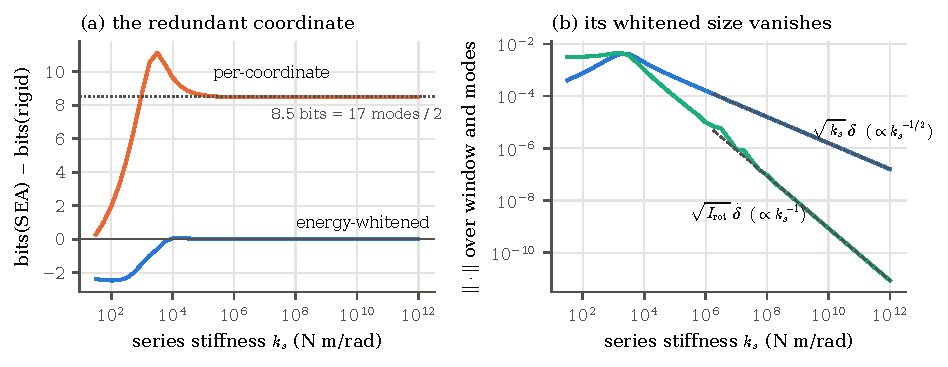
\includegraphics[width=\linewidth]{figures/stiff_limit.pdf}
\caption{(a) Bits of the SEA minus bits of the rigid leg ($B_w=100$\,Hz, $d=17$).
Energy-whitened bits converge to the rigid leg's (the gap is $2.3\times10^{-5}$ bits at
$k_s=10^8$). Per-coordinate bits converge to $8.4716$ bits above it, exactly the
duplicate-readout gain of \cref{prop:dup}. (b) The whitened size of the redundant
direction, summed over samples and input modes. $\sqrt{k_s}\,\delta$ falls with fitted
slope $-0.500$, as \cref{prop:sea} predicts. $\sqrt{I_{\rm rot}}\,\dot\delta$ falls with
slope $-1.009$, faster than the bound, because $\bar a$ is smooth and one more integration
by parts gains another factor $k_s^{-1/2}$.}
\label{fig:stiff}
\end{figure}

\paragraph{Why per-coordinate noise fails, exactly.} For the readout $\Lambda=\diag(1,1,
\omega_{\rm ref}^{-2},\omega_{\rm ref}^{-2})$ (the code's \code{"state"}),
$V^\top\Lambda_qV=2$ and $V^\top\Lambda_vV=2/\omega_{\rm ref}^2$. These are \emph{twice}
the rigid leg's per-coordinate weights. By \cref{thm:limit} the stiff SEA is therefore the
rigid leg observed twice with independent noise, and by \cref{prop:dup} that is worth
$\frac12\sum_i\log_2\frac{1+2\lambda_i}{1+\lambda_i}=8.4716$ bits.

The numerical limit in \cref{fig:stiff}a is $8.4716$ bits, the same number to four
decimals. This is the ``stale'' 8.46 bits pinned in
\code{test\_a\_locked\_series\_spring\_is\_informationally\_a\_rigid\_transmission}, now
derived rather than observed.

\paragraph{The finite-$k_s$ excess is real.} Away from the limit, the spring stores energy
($\sqrt{k_s}\,\delta$ peaks near $k_s\approx3\times10^3$, \cref{fig:stiff}b), and a second
mode enters the force band.
\begin{itemize}[nosep]
  \item At the paper's $B_w=200$\,Hz the energy-whitened gap is $+4.74$, $+7.03$ and
        $+8.57$ bits at $k_s=70$, $10^3$ and $10^4$ (second mode at 190.6\,Hz), and
        $-0.02$ bits at $10^5$. This is the peak in the paper's Fig.~1.
  \item These bits are carried by energy the body really stores. By \cref{lem:energy}
        the whitened size of the spring direction is $\sqrt{k_s}\,\delta$, the square
        root of twice the energy the spring stores. At finite $k_s$ that energy is not
        zero, so the spring direction is a genuine observation, not a copy. As
        $k_s\to\infty$ it vanishes, and with it the extra bits (\cref{thm:limit}).
\end{itemize}

\subsection{How the noise scale enters: two regimes}

\begin{proposition}[Low- and high-SNR asymptotics]\label{prop:snr}
Write the Gram as $G=\sigma^{-2}G_0$, where the noise-free part
$G_0=\sigma_w^2\sum_kX_k^\top\Em X_k$ has eigenvalues $\lambda_1\ge\dots\ge\lambda_d\ge0$,
$r$ of them positive. In this proposition only, write $\gamma=\sigma^{-2}$ for the
precision.
\begin{enumerate}[label=(\alph*)]
  \item \emph{Low SNR (energy regime):}
        $\bits(G)\le\frac{\gamma\tr G_0}{2\ln2}$, with equality to first order in
        $\gamma$. Moreover
        \[
          \frac{\gamma\tr G_0}{2\ln2}
          =\frac{1}{\sigma^2\ln2}\sum_k\E_w\big[\mathcal V(t_k)\big],
        \]
        where $\mathcal V(t)$ is the stored mechanical energy. At low SNR, the bits
        \emph{are} an energy budget: expected stored energy summed over samples, in units
        of $\sigma^2\ln2$.
  \item \emph{High SNR (counting regime):}
        $\bits(G)=\frac r2\log_2\gamma+\frac12\sum_{i\le r}\log_2\lambda_i+o(1)$ as
        $\gamma\to\infty$.
  \item \emph{Consequence for design comparisons.} If designs A and B have the same
        number $r$ of excited modes, their gap tends to
        $\frac12\log_2(\det_+G_{0,A}/\det_+G_{0,B})$, which is \emph{independent of
        $\sigma$}. If $r_A\neq r_B$, the gap grows like $\frac12(r_A-r_B)\log_2\gamma$,
        and the noise scale decides it.
\end{enumerate}
\end{proposition}
\begin{proof}
(a) Write $\bits=\frac12\sum_i\log_2(1+\gamma\lambda_i)$. Use $\log_2(1+u)\le u/\ln2$,
with equality to first order at $u=0$. Then compute
$\tr G_0=\sigma_w^2\sum_k\tr(X_k^\top\Em X_k)=\sum_k\E_w|\Em^{1/2}X_kw|^2$, since
$\E[ww^\top]=\sigma_w^2I$. By \cref{lem:energy} the last expression is
$2\sum_k\E_w\mathcal V(t_k)$.

(b) For $\lambda_i>0$,
$\log_2(1+\gamma\lambda_i)-\log_2(\gamma\lambda_i)=\log_2(1+1/(\gamma\lambda_i))\to0$.
Zero eigenvalues contribute nothing.

(c) Subtract the expansions in (b).
\end{proof}

\checked{Rigid leg vs SEA at $k_s=10^4$ ($B_w=100$\,Hz):
\begin{itemize}[nosep]
  \item both Grams have full rank 17, with condition numbers 26.5 and 29.4;
  \item the predicted high-SNR gap is $\frac12\log_2\det$-ratio $=0.0494$ bits;
  \item the computed gap is $0.0494$ bits for every $\sigma/\sigma_{\rm ref}\le1$, peaks
        at $0.057$ in the crossover, and decays to 0 at low SNR, as (a) requires
        (\cref{fig:snr}).
\end{itemize}
This is why \code{test\_the\_comparison\_does\_not\_ride\_on\_the\_precision\_anchor} passes:
absolute bits move from 191 to 1, but the gap stays put.}

\begin{figure}[t]\centering
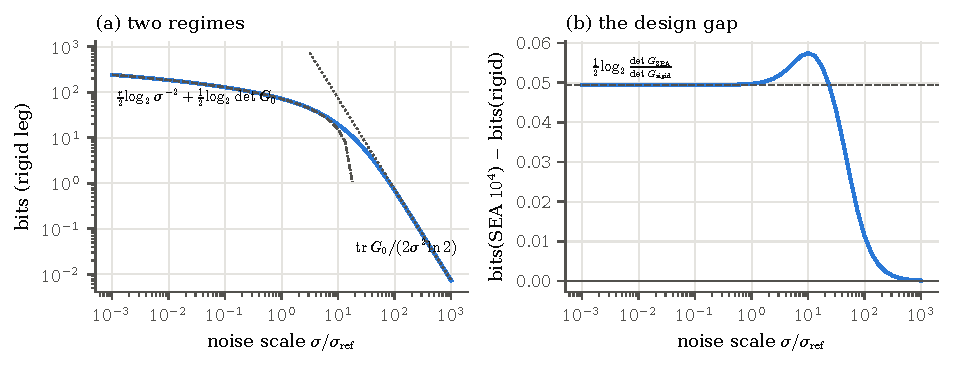
\includegraphics[width=\linewidth]{figures/snr.pdf}
\caption{(a) Bits of the rigid leg against the noise scale, with the high-SNR counting
asymptote (dashed) and the low-SNR energy asymptote (dotted) of \cref{prop:snr}. (b) The
SEA($10^4$) minus rigid gap equals the $\sigma$-independent log-determinant ratio
throughout the high-SNR regime.}
\label{fig:snr}
\end{figure}

\begin{remark}[Sampling rate]\label{rem:fs}
Noise is i.i.d.\ per sample, so one might fear that raising $f_s$ adds bits for free, as
in \cref{prop:dup}. Whether it does depends on how the force prior scales with $f_s$.
\begin{itemize}[nosep]
  \item \emph{The repository's convention is consistent.} The DCT modes are unit-norm
        over the samples (\code{mode\_basis}), so a coefficient's force amplitude scales
        as $f_s^{-1/2}$, while the number of samples scales as $f_s$. The Gram becomes a
        Riemann sum for $\int_0^T x(t)^\top\Em x(t)\,dt$, and bits converge as $f_s$
        grows: $71.62\to71.72\to71.77$ bits at 2, 4 and 8\,kHz (rigid leg).
  \item \emph{The inconsistent alternative.} Holding the force waveform fixed instead
        adds $8.5$ bits per doubling: $63.18\to71.72\to80.24$. This is the
        duplicate-readout artifact in time.
  \item \emph{The design gap is unaffected} in both conventions (equal rank,
        \cref{prop:snr}c).
  \item A revision should state that the $\varphi_j$ are orthonormal over samples, or
        equivalently specify the force prior in continuous $L^2$ (\code{check\_sampling}).
\end{itemize}
\end{remark}

%=========================================================================================
\section{Attribution and morphological computation}
\label{sec:shapley}

\subsection{A consistent noise model for subsets of coordinates}

The paper's Eq.~(10) attributes bits to coordinates using
$\nu(S)=I(W;X_S)$. What noise does $X_S$ carry? The repository
(\code{spectrum.coordinate\_bits}) uses the marginal $(\sigma^2\Em^{-1})_{SS}$ with a
pseudo-inverse. The following makes the reason precise; the paper should state it.

\begin{definition}[Observing a subset]\label{def:subset}
The noise lives on the \emph{body}, not on a sensor: $\tilde x_q=x_q+\nu$ with
$\nu\sim\mathcal N(0,\sigma^2\Em^{-1})$ independently at each sample. Observing a subset
$S$ of coordinates means observing $P_S\tilde x_q$, where $P_S$ selects rows. Its noise
covariance is $N_S=\sigma^2(\Em^{-1})_{SS}$.
\end{definition}

\begin{proposition}[Properties of the subset game]\label{prop:subset}
With $\nu(S)$ the information in $\{P_S\tilde x_q(t_k)\}_k$:
\begin{enumerate}[label=(\alph*)]
  \item \emph{Consistency:} $\nu(\text{all coordinates})$ equals the energy-whitened total.
  \item \emph{Monotonicity:} $S\subseteq S'$ implies $\nu(S)\le\nu(S')$. Hence every
        Shapley value is nonnegative, and they sum to the total (efficiency).
  \item \emph{Exact duplicates are worth one copy:} if coordinate $b$'s signal \emph{and}
        noise are almost surely equal to coordinate $a$'s, then $\nu(S\cup\{a,b\})=
        \nu(S\cup\{a\})=\nu(S\cup\{b\})$ for every $S$. Hence $\phi_a=\phi_b$, and the
        pair together earns what one of them earns.
  \item \emph{Independent duplicates fuse by precision:} if $y_a=v+n_a$ and $y_b=v+n_b$
        with $n_a,n_b$ independent of each other and of $v$, with variances $s_a^2$ and
        $s_b^2$, then $(y_a,y_b)$ carries exactly the information of one observation
        $v+\hat n$ with $1/\Var\hat n=1/s_a^2+1/s_b^2$.
\end{enumerate}
\end{proposition}
\begin{proof}
(a) With $S$ everything, $N_S=\sigma^2\Em^{-1}$ is invertible. The Gaussian formula with
colored noise uses the weight $N_S^{-1}=\Em/\sigma^2$, which is \eqref{eq:gram} with
$C^\top C=\Em$.

(b) $P_S\tilde x_q$ is a sub-vector of $P_{S'}\tilde x_q$, hence a function of it, and
data processing applies. Every marginal contribution
$\nu(S\cup\{i\})-\nu(S)$ is therefore $\ge0$, so every Shapley value, being a weighted
average of these, is $\ge0$. Efficiency is a standard property of the Shapley value.

(c) If $y_b=y_a$ almost surely, then $(y_S,y_a,y_b)$ and $(y_S,y_a)$ are functions of
each other, so they carry the same information; the same holds with $a$ and $b$
swapped. The two players are interchangeable in every coalition, so the symmetry axiom
gives $\phi_a=\phi_b$.

On the code side: the noise covariance of the pair is singular, $s^2\left[\begin{smallmatrix}1&1\\1&1
\end{smallmatrix}\right]$. Its pseudo-inverse $\frac1{4s^2}\left[\begin{smallmatrix}1&1\\1&1\end{smallmatrix}
\right]$, applied to the signal $(m,m)$, gives $m^2/s^2$, which is exactly the
single-copy value. The pseudo-inverse thus computes the correct information on the range
of the noise.

(d) Let $\hat v=(y_a/s_a^2+y_b/s_b^2)/(1/s_a^2+1/s_b^2)$ and $u=y_a-y_b=n_a-n_b$.
\begin{itemize}[nosep]
  \item The map $(y_a,y_b)\mapsto(\hat v,u)$ is invertible.
  \item $u$ does not involve $v$.
  \item $\Cov(\hat v,u)\propto s_a^2/s_a^2-s_b^2/s_b^2=0$, so the jointly Gaussian pair
        $(\hat v-v,u)$ is independent, and $u$ is independent of $(v,\hat v)$.
\end{itemize}
Therefore $I(v;y_a,y_b)=I(v;\hat v,u)=I(v;\hat v)$, and
$\hat v=v+\hat n$ with $\Var\hat n=(1/s_a^2+1/s_b^2)^{-1}$.
\end{proof}

\paragraph{The stiff SEA has one redundancy of each kind.}
\begin{itemize}
  \item \emph{Positions are exact duplicates in the limit.} The position noise is
        $\sigma^2K_\kappa^{-1}$. As $k_s\to\infty$, the correlation of the noises on
        $\theta_j$ and $\theta_m$ goes to 1: it is $0.08$, $0.30$, $0.71$, $0.995$ and
        $0.99995$ at $k_s=70$, $10^3$, $10^4$, $10^6$ and $10^8$. The signals coincide
        too. By (c) the two positions earn equal Shapley credit, $22.948$ and $22.947$
        bits at $k_s=10^8$, and together they earn what the rigid leg's single angle earns
        (66.836 bits, both).
  \item \emph{Velocities are independent duplicates.} $H$ is diagonal, so the velocity
        noise $\sigma^2H^{-1}$ is \emph{uncorrelated}, with precisions $m_lr^2/\sigma^2$
        and $I_{\rm rot}/\sigma^2$. By (d) they fuse into one observation with precision
        $(m_lr^2+I_{\rm rot})/\sigma^2$, which is \emph{exactly the rigid leg's velocity
        precision}, $H_V/\sigma^2$. Numerically, the pair gives 51.216 bits, as does the
        rigid leg's velocity.

        The players are \emph{not} symmetric: $\dot\theta_j$ carries three times the
        precision of $\dot\theta_m$ ($m_lr^2=0.03$ vs $I_{\rm rot}=0.01$). Its Shapley
        share is correspondingly larger, $15.60$ vs $10.23$ bits.
\end{itemize}
The paper's Fig.~2 text says the coordinates ``are redundant at high stiffness, and so
give equal Shapley contributions.'' That is exact for positions. For velocities the
credit is split by inertia (\cref{fig:shapley}). Both mechanisms are the restriction
property of \cref{lem:restrict} at work on subsets.

\begin{figure}[t]\centering
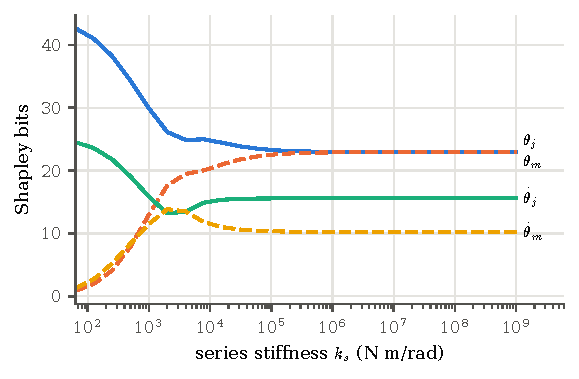
\includegraphics[width=0.62\linewidth]{figures/shapley.pdf}
\caption{Shapley bits per SEA coordinate against $k_s$ ($B_w=100$\,Hz). Positions converge
to equal shares, because their noise becomes perfectly correlated. Velocities converge to
unequal shares fixed by the inertia ratio, because their noise stays independent and fuses
by precision (\cref{prop:subset}).}
\label{fig:shapley}
\end{figure}

\subsection{Morphological computation \texorpdfstring{$\mathrm{MC}_W$}{MCW}}
\label{sec:mcw}

\citet{zahedi2013quantifying} define $\mathrm{MC}_W=I(W';W\mid A)$ for discrete variables
estimated from visited states. They do not assume an equilibrium distribution (we could
read this only through secondary sources; \cref{app:sources}).

The repository's linear version (\code{channel.morphological\_bits}) is a modelling
addition. It takes the state law to be the Gibbs law $\Em^{-1}$ and chooses the one-step
process noise $Q=P-A_dPA_d^\top$ so that $P$ is stationary, with $A_d=e^{A\Delta t}$.

\begin{proposition}[Closed form, and when it exists]\label{prop:mcw}
Let $\At_d=\Em^{1/2}A_d\Em^{-1/2}$ with singular values $s_i$.
\begin{enumerate}[label=(\alph*)]
  \item $Q\succeq0$ if and only if $\|\At_d\|_2\le1$, and this always holds by
        \cref{thm:ph}(b), since $\At_d=e^{\At\Delta t}$.
  \item Without action conditioning,
        \[
          \mathrm{MC}_W=I(x_{k+1};x_k)=-\tfrac12\log_2\det\big(I-\At_d\At_d^\top\big)
          =-\tfrac12\sum_i\log_2(1-s_i^2).
        \]
\end{enumerate}
\end{proposition}
\begin{proof}
Mutual information is invariant under the invertible maps $x\mapsto\Em^{1/2}x$
(\cref{lem:noise}a), so we may work in whitened coordinates.

(a) There $P$ becomes $I$, and $Q$ becomes $\tilde Q=I-\At_d\At_d^\top$.
$\tilde Q\succeq0$ exactly when every singular value of $\At_d$ is at most 1.

(b) In whitened coordinates, $\tilde x_{k+1}=\At_d\tilde x_k+\tilde n$ with
$\Cov\tilde x_k=I$ and $\Cov\tilde n=\tilde Q$. Hence $\Cov\tilde x_{k+1}=\At_d\At_d^\top+
\tilde Q=I$, and
\[
  I=\tfrac12\log_2\frac{\det\Cov\tilde x_{k+1}}{\det\Cov\tilde n}
   =-\tfrac12\log_2\det\tilde Q .
\]
\end{proof}

\phys{$\mathrm{MC}_W$ measures how close the whitened one-step map is to an \emph{isometry}.
Each lightly damped direction ($s_i\to1$) contributes $-\frac12\log_2(1-s_i^2)$, which is
large. In plain terms, $\mathrm{MC}_W$ rewards \emph{undissipated stored energy}: memory.

For the SEA: an extra mode with series damping ratio $\zeta_s=0.1$ adds a nearly
isometric direction. The largest $s_i$ is $0.99999985$ at $k_s=70$ and $0.99995$ for the
rigid leg. So $\mathrm{MC}_W$ is $22.22$ bits (SEA, $k_s=70$) vs $8.56$ bits (rigid),
falling to $9.61$ bits at $k_s=10^6$. The closed form matches the code to $10^{-9}$
(\code{check\_mcw\_closed\_form}).

This is the mechanism behind the tension in the paper's Sec.~VI. $I(W;X)$ rewards
\emph{transmitting force into} the state; $\mathrm{MC}_W$ rewards \emph{keeping} energy in
the state. A compliant, lightly damped body does more of the second and, at stiff contact,
less of the first. The closed form also explains why $\mathrm{MC}_W$ diverges as
$\Delta t\to0$ ($s_i=1-O(\zeta_i\omega_i\Delta t)$) and why it requires $\Em\succ0$
(\cref{sec:floating}).}

%=========================================================================================
\section{Related problems the energy metric solves}
\label{sec:related}

\subsection{Continuum and soft bodies: independence from the mesh}

Soft robots and compliant links are modelled by finite elements, where the number of
coordinates is a numerical choice. A sound information measure must converge as the mesh
is refined.

\begin{theorem}[Mesh independence]\label{thm:mesh}
Let a linear elastic body be semi-discretized by conforming finite elements, with
consistent mass $H_N$ and stiffness $K_N$, and let $u_N(t)$ be the finite-element field. Then the
energy-whitened Gram is
\[
  G_N^{ij}=\gamma\sum_k\Big[a\big(u^i_{N,k},u^j_{N,k}\big)+m\big(\dot u^i_{N,k},\dot u^j_{N,k}\big)\Big],
\]
where $a(\cdot,\cdot)$ is the continuum strain-energy bilinear form and $m(\cdot,\cdot)$ the
continuum kinetic-energy (mass) form. Suppose the finite-element solutions converge in the
energy norm at each sample time. This is classical for semi-discrete approximations of
damped second-order hyperbolic problems with sufficiently regular data
\citep{dupont1973l2,baker1976error,geveci1984convergence}; we \emph{assume} it here. Then
$G_N\to G_\infty$ and the bits converge.

By contrast, per-node isotropic noise has Gram entries
$\approx\frac{N}{L}\times(L^2\text{ inner product})$. It grows linearly in $N$, so by
\cref{prop:snr}b the bits grow like $\frac r2\log_2N$: about $\frac r2$ bits per mesh
doubling.
\end{theorem}
\begin{proof}
\emph{The identity.} With $u_N=\sum_iU_i\psi_i$ in the nodal basis, the finite-element
matrices are defined by $U^\top K_NU'=a(u_N,u_N')$ and $\dot U^\top H_N\dot U'=m(\dot
u_N,\dot u_N')$. Substituting into \eqref{eq:gram} with $C^\top C=\Em_N$ gives the
displayed identity. The nodes have disappeared: the Gram is a sum of \emph{continuum}
energy inner products of the finite-element fields.

\emph{Convergence.} Each entry is a finite sum (over finitely many $k$) of inner products,
which are continuous in the energy norm. So energy-norm convergence of each field implies
convergence of each entry. Then apply continuity of $\log\det(I+\cdot)$.

\emph{The per-node estimate.} For a uniform mesh of spacing $h=L/N$ and smooth fields,
$\sum_iU_iU_i'\approx h^{-1}\int uu'\,dx$, a Riemann sum.
\end{proof}

\begin{remark}[Cylindrical noise is harmless here]
In the continuum limit, isotropic noise in energy coordinates is white noise on the energy
Hilbert space. That is a cylindrical measure, not a countably additive one. It does no
harm here: the signal $\{Mw\}$ spans at most $d$ dimensions, and \cref{lem:gauss} shows
that the information depends only on the $d\times d$ matrix $M^\top M$. This is the
noise-side counterpart of the requirement, stressed in function-space Bayesian inversion,
that priors and inner products be defined so as to survive refinement:
\begin{itemize}[nosep]
  \item MCMC proposals that are robust under mesh refinement
        \citep{cotter2013mcmc};
  \item finite-element inner products weighted by the mass matrix
        \citep[Sec.~3.3]{buithanh2013computational};
  \item see also \citet{stuart2010inverse}.
\end{itemize}
\end{remark}

\checked{A fixed--free axial rod (length 0.2\,m, $EA=10^3$\,N, $\rho A=0.1$\,kg/m, so the
first mode is at 125\,Hz) with consistent mass, stiffness-proportional damping and a tip
force ($B_w=400$\,Hz, $d=68$), for $N=2,\dots,128$ elements (\cref{fig:rod},
\code{check\_rod}):
\begin{itemize}[nosep]
  \item energy-whitened bits converge, $297.93\to302.109$, changing by $0.004$ between
        $N=64$ and $128$;
  \item per-node isotropic bits grow by $33.2$ bits per doubling, against
        $\frac r2=34$ predicted;
  \item a fixed tip sensor (a physical point sensor) also converges, which shows that the
        problem is noise \emph{per coordinate}, not discretization.
\end{itemize}}

\begin{figure}[t]\centering
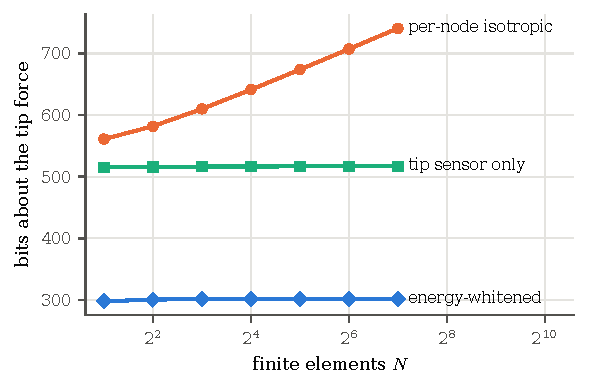
\includegraphics[width=0.62\linewidth]{figures/rod.pdf}
\caption{Mesh refinement of a finite-element rod. Energy whitening gives a
mesh-independent answer. Per-node noise is the duplicate-readout artifact of
\cref{prop:dup} at scale: every refinement adds ``free second looks.''}
\label{fig:rod}
\end{figure}

\subsection{Gear ratios and transmission design}

Relabelling a motor angle on the input side of a gear as an angle on the output side is a
reparametrization: $T=\diag(1,1/N)$ in the SEA layout. By \cref{thm:invariance},
energy-whitened bits do not move. Per-coordinate bits jump from 81.37 to 130.91 bits
(\cref{fig:invariance}).

\emph{Changing} the gear ratio is a different matter: it changes the reflected inertia
$N^2I_{\rm rot}$, which is a physical change in $H$. That change enters $\Em$, and it
correctly changes the bits. The energy metric thus separates bookkeeping from design,
which is what the paper's Table~I rotor-inertia sweep needs.

\subsection{Floating bases: when a singular metric loses nothing}
\label{sec:floating}

For an unclamped leg or a free-flying quadruped, $K$ is singular: rigid-body
\emph{positions} store no energy, while $H\succ0$ still weighs velocities. The
whitened readout $\Em^{1/2}$, with eigenvalues clipped at zero by \code{sym\_sqrt}, is
blind to zero-energy positions. Does that lose information?

\begin{proposition}[No loss when force and ground share the Jacobian]\label{prop:floating}
Suppose:
\begin{enumerate}[label=(\roman*),nosep]
  \item $K\succeq k_iJ^\top J$ with $k_i>0$, where $J$ is the Jacobian through which the
        unknown force acts;
  \item $D\phi=0$ for every $\phi\in\ker K$. Physically, internal and ground dampers act
        only on relative or foot motion.
\end{enumerate}
Then, from rest, the trajectory never enters $\ker K$. More precisely, $\phi^\top Hq(t)=0$
for all $\phi\in\ker K$ and all $t$. On the subspace where the motion lives, $\Em$ is
positive definite, so nothing is lost.
\end{proposition}
\begin{proof}
\emph{Step 1: zero-energy modes are not forced.} For $\phi\in\ker K$,
$0=\phi^\top K\phi\ge k_i(J\phi)^2$, so $J\phi=0$.

\emph{Step 2: their coordinates stay at zero.} Let $\eta=\phi^\top Hq$. Multiply
\eqref{eq:eom} on the left by $\phi^\top$:
\[
  \ddot\eta=(J\phi)^\top f-(D\phi)^\top\dot q-(K\phi)^\top q=0 .
\]
With $\eta(0)=\dot\eta(0)=0$, we get $\eta\equiv0$.

\emph{Step 3: $\Em$ is definite on the motion.} By Step 2, $q(t)$ lies in the
$H$-orthogonal complement of $\ker K$. Any nonzero $q$ in that complement is not in
$\ker K$, so $q^\top Kq>0$ there.
\end{proof}

\checked{On the repository's free bench (trunk plus leg, $q=(y_b,\theta)$), the
energy-whitened and \code{"kinetic"} ($\omega_{\rm ref}^2H$) readouts give the same bits,
71.709.

This equality is not a coincidence. The motion lives on $\mathrm{span}(H^{-1}J^\top)$. On
that line, $K$ restricts to $k_i(JH^{-1}J^\top)^2$ and $H$ restricts to $JH^{-1}J^\top$.
Their ratio is $k_i/m_e=\omega_{\rm ref}^2$, where $m_e$ is the effective mass at the foot,
so the two metrics agree on the motion.

A counterexample violates (i) by pushing on the trunk instead of the foot. The zero mode
is then forced ($\phi_0^\top e_1=-0.17$), and the singular metric loses
$71.86-49.66=22.2$ bits relative to the regularized one (\code{check\_floating}).}

\phys{The paper's Sec.~V applies random pushes $w_{\rm ext}$ to the calves of a floating
quadruped. Those pushes do excite zero-stiffness base positions, so an energy metric built
from joint springs alone would discard base-position information. Three remedies:
\begin{enumerate}[nosep]
  \item keep the base velocities (always weighted, since $H\succ0$) and accept that base
        position is gauge;
  \item regularize the position block with $\omega_{\rm ref}^2H$ (the code's
        \code{"kinetic"} readout) and report sensitivity to $\omega_{\rm ref}$;
  \item use the potential of gravity and contact springs at the operating point.
\end{enumerate}
The Zahedi--Ay $\mathrm{MC}_W$ of \cref{sec:mcw} has no Gibbs law when $\Em$ is singular,
which is why \code{morphological\_bits} correctly refuses the free bench.}

\subsection{Further uses}
\begin{itemize}
  \item \emph{Sensor placement.} \Cref{def:subset} turns ``where should the encoder go?''
        into a Bayesian D-optimal design over physical sensor sites, with noise attached
        to the body. This is the energy-consistent analogue of effective independence
        \citep{kammer1991sensor,papadimitriou2004optimal}. Joint-side vs motor-side
        sensing on the SEA (\cref{fig:shapley}) is the simplest instance.
  \item \emph{Variable-stiffness and parallel-elastic actuators, compliant feet.} All of
        these add or remove coordinates as parameters vary. \Cref{thm:limit} guarantees
        continuity across the degenerate limits.
  \item \emph{Learned estimators.} For InfoNCE, whitening does not change the true
        information (\cref{lem:noise}a), but it gives the critic dimensionally
        homogeneous inputs in $\sqrt{\mathrm J}$. Per-feature $z$-scoring is a
        data-dependent diagonal metric: it is not basis-free, and it changes with the
        force prior. Noise must be added \emph{after} whitening, as \code{sim\_info} does.
\end{itemize}

%=========================================================================================
\section{Part II. Is energy the right choice?}
\label{sec:right}

Sections~\ref{sec:setup}--\ref{sec:related} (Part~I) took the energy metric as given and showed what it does. This part asks whether it
is the right choice for measuring mechanical intelligence, and what it leaves out.

\subsection{What maximum entropy does and does not decide}

The proof of \cref{thm:maxent} never uses the fact that $\Em$ is an energy. For \emph{any}
positive-definite form $W$, the same three steps show that the maximum-entropy law under
$\E[\nu^\top W\nu]=m\sigma^2$ is $\mathcal N(0,\sigma^2W^{-1})$. So maximum entropy turns
a choice of \emph{what is held fixed} into a noise law. It does not make that choice.

For example, constraining the mean \emph{action}, i.e.\ each mode's energy divided by its
frequency, gives the action-weighted law. That is the shape of quantum zero-point noise
(\cref{rem:quantum}). The real modeling assumption is ``resolution is measured in
energy.'' The rest of this section justifies that assumption from properties a noise model
should have.

\subsection{Five requirements, and a uniqueness theorem}

\begin{definition}[Mechanisms and noise rules]\label{def:rule}
A mechanism is assembled from single-parameter elements:
\begin{itemize}[nosep]
  \item \emph{springs}: stiffness $k_e$ acting on a relative coordinate $s_e=a_e^\top q$;
  \item \emph{inertias}: a positive-definite inertia matrix $M_m$ acting on a velocity
        $u_m=B_m\dot q$;
  \item \emph{dampers}: coefficient $b_e$ acting on $\dot s_e$.
\end{itemize}
Hence $K=\sum_ek_ea_ea_e^\top$, $H=\sum_mB_m^\top M_mB_m$ and $D=\sum_eb_ea_ea_e^\top$.
A \emph{noise rule} assigns to every mechanism a positive-semidefinite quadratic form
$W(q,\dot q)$, the precision of the body's resolution: noise $\mathcal N(0,\sigma^2W^{-1})$.
\end{definition}

The requirements, each with the reason it matters:
\begin{enumerate}[label=(U\arabic*)]
  \item \emph{Coordinate-free.} $W$ transforms with the coordinates
        ($\tilde W=\mathcal T^\top W\mathcal T$ under $q=T\tilde q$), including rescalings of
        each element's own coordinate. Otherwise relabeling changes the answer
        (\cref{thm:invariance}).
  \item \emph{Local and universal.} $W$ is a sum of one term per element. Each term depends
        only on that element's parameter and kinematics, through a function fixed for each
        element type. Adding a component somewhere must not change how precisely another
        component's state is known; this is what makes components compose, stiff limits
        behave (\cref{thm:limit}) and meshes converge (\cref{thm:mesh}). Universality says
        the rule cannot know which spring is which.
  \item \emph{No outside scales.} No dimensional constant other than the element's own
        parameter may appear: no reference frequency, length or time. Otherwise the result
        depends on an arbitrary choice; the \code{"kinetic"} readout's $\omega_{\rm ref}$
        can flip the sign of the SEA--rigid comparison
        (\code{test\_the\_ground\_decides\_whether\_series\_compliance\_helps\_or\_hurts}).
  \item \emph{Time-reversal symmetric.} $W(q,-\dot q)=W(q,\dot q)$. Resolution should not
        depend on the direction of motion.
  \item \emph{Unchanged by free motion.} For every mechanism without dampers, $W$ is
        constant along every solution of $H\ddot q+Kq=0$. \Cref{prop:work} shows this is
        exactly the requirement that free motion never creates information.
\end{enumerate}

\begin{theorem}[Uniqueness of the energy metric]\label{thm:unique}
A noise rule satisfies (U1)--(U5) if and only if
$W=c\,(q^\top Kq+\dot q^\top H\dot q)=c\,x_q^\top\Em x_q$ for a constant $c>0$, i.e.\ it is
the energy metric up to the overall noise scale.
\end{theorem}
\begin{proof}
\emph{The energy metric satisfies all five.}
\begin{itemize}[nosep]
  \item (U1) is \cref{thm:invariance}.
  \item (U2)--(U4) hold by inspection: $k_es_e^2$ and $u_m^\top M_mu_m$ are energies.
  \item (U5) holds because energy is conserved without damping:
        $\frac{d}{dt}(q^\top Kq+\dot q^\top H\dot q)=2\dot q^\top(Kq+H\ddot q)=0$.
\end{itemize}

\emph{Conversely, step 1: a spring.} By (U2) its term is a quadratic form in its own
kinematics $(s,\dot s)$ with coefficients depending only on $k$:
$\alpha_1(k)s^2+\alpha_2(k)s\dot s+\alpha_3(k)\dot s^2$.
\begin{itemize}[nosep]
  \item (U4) gives $\alpha_2=0$.
  \item Rescaling the spring's coordinate, $s=\lambda\tilde s$, turns the stiffness into
        $\tilde k=\lambda^2k$. By (U1) the term must keep its value:
        $\alpha_1(\lambda^2k)\tilde s^2=\alpha_1(k)\lambda^2\tilde s^2$ for every
        $\lambda>0$, so $\alpha_1(k)=\alpha\,k$ for a dimensionless constant $\alpha$.
        Likewise $\alpha_3(k)\propto k$.
  \item But $k\dot s^2$ has units of energy times time squared. Turning it into an energy
        needs a time scale, which (U3) forbids. So $\alpha_3=0$, and the spring's term is
        $\alpha\,k_es_e^2$.
\end{itemize}

\emph{Step 2: an inertia.} Its kinematics is a velocity $u$, and a position-dependent term
would need a time scale (U3). So its term is $u^\top F(M)u$ for some matrix function $F$.
\begin{itemize}[nosep]
  \item (U1), applied to a change of the element's velocity coordinates $u=T\tilde u$
        (which sends $M\mapsto T^\top MT$), requires $F(T^\top MT)=T^\top F(M)T$ for every
        invertible $T$.
  \item Taking $T=M^{-1/2}$ gives $F(M)=M^{1/2}F(I)M^{1/2}$.
  \item Taking $T$ orthogonal gives $F(I)=T^\top F(I)T$ for every orthogonal $T$, so
        $F(I)=\beta I$ (a matrix that commutes with all rotations is a multiple of the
        identity).
  \item Hence the term is $\beta\,u_m^\top M_mu_m$.
\end{itemize}

\emph{Step 3: a damper.} The same rescaling argument makes any term proportional to $b$.
The candidates are $b\,s\dot s$, $b\,s^2$ and $b\,\dot s^2$:
\begin{itemize}[nosep]
  \item $b\,s\dot s$ is odd in time, which (U4) forbids;
  \item $b\,s^2$ has units of energy times time, and $b\,\dot s^2$ is a power; turning
        either into an energy needs a time scale, which (U3) forbids.
\end{itemize}
Dampers therefore contribute nothing.

\emph{Step 4: free motion fixes the ratio.} By universality ((U2)) the constants $\alpha$
and $\beta$ are the same for every element, so $W=\alpha\,q^\top Kq+\beta\,\dot q^\top
H\dot q$. Along any solution of $H\ddot q=-Kq$,
\[
  \tfrac{d}{dt}W=2\alpha\,\dot q^\top Kq+2\beta\,\dot q^\top H\ddot q
  =2(\alpha-\beta)\,\dot q^\top Kq .
\]
For any mechanism with a spring, some state has $\dot q^\top Kq\neq0$, so (U5) forces
$\alpha=\beta=:c$.
\end{proof}

\begin{remark}[What the axioms do and do not exclude]
\begin{itemize}[nosep]
  \item \emph{Elements are single constitutive laws.} A Kelvin--Voigt element (spring and
        damper as one element) has an internal time scale $b/k$. If it were treated as one
        element, (U3) would allow a term $(b^2/k)\dot s^2$. Treating springs and dampers as
        separate elements, as their additive force laws suggest, removes this.
  \item \emph{Universality matters.} Without it, (U5) still forces $\alpha=\beta$, but only
        within each mechanically connected component. Two disconnected bodies could carry
        different noise scales.
  \item \emph{Dissipation drops out by itself.} No assumption singled out damping; the
        axioms exclude it from the metric.
\end{itemize}
\end{remark}

\checked{The identity $\frac{d}{dt}W=2(\alpha-\beta)\dot q^\top Kq$ holds to
$4\times10^{-14}$ on random SEA states (\code{check\_uniqueness\_flow}). Over 20\,ms of
undamped SEA motion, the deviation of $\Phi^\top W\Phi$ from $W$ is $4\times10^{-13}$ for
the energy and the frequency-weighted forms of \cref{sec:alternatives}, but $6.4$ for
per-coordinate noise and $1.7$ for the kinetic metric (relative to $\max|W|$;
\code{check\_flow\_invariance}).}

\subsection{Free motion cannot create information}

The fifth requirement looks like a technicality. It is the most important one for
attributing computation to a body.

\begin{proposition}[Information is created only by work]\label{prop:work}
Store information about a random variable $Y$ in the body's state, $x(0)$, and let the
body move freely ($f=0$). Observe $x(t)$ through physical noise $\nu\sim\mathcal
N(0,\sigma^2W^{-1})$ independent of $Y$, and let $I_t=I(Y;x(t)+\nu)$. Write $\Phi(t)$ for
the state-transition matrix.
\begin{enumerate}[label=(\roman*)]
  \item If $D=0$ and $\Phi^\top W\Phi=W$ (for example $W=\Em$), then $I_t=I_0$ for all
        $t$.
  \item If $W=\Em$ and $D\succeq0$, then $I_t$ is non-increasing in $t$.
  \item If $D=0$ and $\Phi(t)^\top W\Phi(t)\neq W$ for some $t$, then there is a Gaussian
        scalar $Y$ with $I_t>I_0$: free motion creates apparent information.
\end{enumerate}
Consequently, among quadratic noise models, (U5) holds \emph{if and only if} free
conservative motion never creates information.
\end{proposition}
\begin{proof}
Work in the coordinates $z=W^{1/2}x$, where the noise is $\mathcal N(0,\sigma^2I)$ and the
flow is $\tilde\Phi=W^{1/2}\Phi W^{-1/2}$. Note that
$\tilde\Phi^\top\tilde\Phi=W^{-1/2}\Phi^\top W\Phi W^{-1/2}$.

(i) If $\Phi^\top W\Phi=W$, then $\tilde\Phi$ is orthogonal. The observation
$\tilde\Phi z(0)+n$ is an invertible transformation of $z(0)+\tilde\Phi^\top n$, and
$\tilde\Phi^\top n\sim\mathcal N(0,\sigma^2I)$ has the same law as $n$. So the two
observations carry the same information about $Y$ (\cref{lem:noise}a).

(ii) With $W=\Em$, $\tilde\Phi(s)=e^{\At s}$ is a contraction, $\|C\|_2\le1$, by
\cref{thm:ph}(b). Fix $t$ and $s\ge0$, and let $C=e^{\At s}$, so that
$z(t+s)+n=Cz(t)+n$. Let $n_1\sim\mathcal N(0,\sigma^2I)$ and $n_2\sim\mathcal
N(0,\sigma^2(I-CC^\top))$ be independent; the second covariance is valid because
$\|C\|\le1$. Then $C(z(t)+n_1)+n_2$ has noise covariance
$\sigma^2(CC^\top+I-CC^\top)=\sigma^2I$, so it has the same joint law with $Y$ as
$Cz(t)+n$. It is obtained from the earlier observation $z(t)+n_1$ by further processing
plus independent noise. By the data-processing inequality, $I_{t+s}\le I_t$.

(iii) Let $R=\tilde\Phi^\top\tilde\Phi\neq I$; it is symmetric positive definite.
Liouville's theorem gives $\det\Phi(t)=e^{t\,\tr A}=1$, because $\tr A=-\tr(H^{-1}D)=0$
when $D=0$. Hence $\det R=\det(\Phi)^2=1$. A positive-definite matrix with determinant 1
that is not the identity has an eigenvalue $\lambda_{\max}>1$ (eigenvalues whose product
is 1 cannot all be $\le1$ unless all equal 1). Let $u$ be its eigenvector, and store
$Y\sim\mathcal N(0,\sigma_Y^2)$ as $x(0)=W^{-1/2}u\,Y$. Then
\[
  I_0=\tfrac12\log\!\Big(1+\tfrac{\sigma_Y^2}{\sigma^2}|u|^2\Big)
  <\tfrac12\log\!\Big(1+\tfrac{\sigma_Y^2}{\sigma^2}\lambda_{\max}|u|^2\Big)=I_t .
\]
\end{proof}

\phys{Under the energy metric, a body's information about anything it has stored can change
in only two ways: the force does work on it, which can add information, or the dampers
dissipate it, which can only remove information. Conservative motion merely moves
information around, as a rotation in whitened coordinates.

Under any other quadratic noise model, a free oscillation that rotates the state into
better-resolved directions creates bits from nothing. A measure of mechanical computation
should credit the body for what the force delivered and debit it for what was dissipated,
not for coordinate artifacts of free motion. This is the same accounting as in the
thermodynamics of computation \citep{landauer1961irreversibility,bennett1982thermodynamics}:
conservative dynamics are reversible and lose nothing, and dissipation is the irreversible
step.}

\begin{figure}[t]\centering
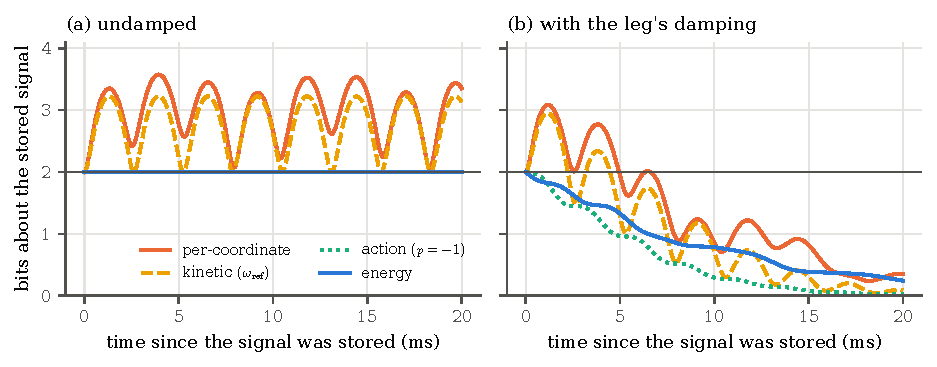
\includegraphics[width=\linewidth]{figures/free_motion.pdf}
\caption{Information about a signal stored in the SEA's state ($k_s=10^4$), under free
motion, for four noise models. Each starts from the direction it resolves worst, scaled to
2 bits. (a) Undamped: energy and action weighting stay at exactly 2 bits. Per-coordinate
noise reaches 3.58 bits and the kinetic metric 3.22 bits, created by free motion alone.
(b) With the leg's damping, energy can only decrease (\cref{prop:work}ii). Per-coordinate
noise still rises to 3.08 bits first (\code{check\_free\_motion}).}
\label{fig:freemotion}
\end{figure}

\begin{remark}[Classical versus quantum: why energy and not action]\label{rem:quantum}
The quantum fluctuation--dissipation theorem \citep{callen1951irreversibility} gives each
mode of frequency $\omega$ a fluctuation energy
$\frac{\hbar\omega}2\coth\frac{\hbar\omega}{2k_BT}$. In whitened coordinates this is the
noise variance per mode.
\begin{itemize}[nosep]
  \item When $k_BT\ll\hbar\omega$ it tends to $\frac12\hbar\omega$: noise energy grows
        with frequency, which is action weighting (precision $\propto1/\omega$).
  \item When $k_BT\gg\hbar\omega$ it tends to $k_BT$: equal energy per mode, the energy
        metric.
\end{itemize}
For a 200\,Hz mode at room temperature, $\hbar\omega/k_BT\approx3\times10^{-11}$, so
macroscopic mechanisms sit deep in the classical regime. Physics and the locality axiom
agree: for robots, the currency of resolution is energy.

Energy is also the additive conserved quantity associated with time-translation symmetry
(Noether), which is why it can be assembled element by element.
\end{remark}

%=========================================================================================
\section{The alternatives compared}
\label{sec:alternatives}

\Cref{tab:rules} lists the candidate noise models, the requirements each violates, and how
it behaves in the two limits of Part~I. The frequency-weighted family is
\[
  W_p=\sum_i\omega_i^p\,(\text{modal energy form } i)
  =\Em^{1/2}\diag\!\big((\Omega\Omega^\top)^{p/2},(\Omega^\top\Omega)^{p/2}\big)\Em^{1/2},
\]
with $\Omega=K^{1/2}H^{-1/2}$ as in \cref{thm:ph}. Here $p=0$ is the energy metric and
$p=-1$ is action weighting. (For numerical comparison each $W_p$ is divided by
$\omega_{\rm ref}^p$ so that it is measured in joules; this constant cancels in every
design gap.)

\begin{table}[t]\centering\small
\caption{Candidate noise models. The stiff-limit column is SEA minus rigid bits at
$k_s=10^{10}$ ($B_w=100$\,Hz). The mesh column is the change from $N=32$ to $N=64$
elements on the rod of \cref{thm:mesh}.}
\label{tab:rules}
\begin{tabular}{>{\raggedright}p{0.25\linewidth}p{0.17\linewidth}>{\raggedright}p{0.17\linewidth}>{\raggedright\arraybackslash}p{0.27\linewidth}}
\toprule
Rule & Violates & Stiff limit (bits) & Mesh, $32\to64$ (bits)\\
\midrule
energy $W_0=\Em$ & --- & $0.0000$ & $+0.017$ (converges)\\
action $W_{-1}$ & U2 & $0.0000$ & $+0.010$ (converges)\\
$W_{+1}$ & U2 & $0.0007$, slowly & $+2.96$ (keeps growing)\\
$W_{+2}$ & U2 & $1.489$ (no limit) & ---\\
$W_{+3}$ & U2 & $60.1$ (diverges) & ---\\
kinetic, $\diag(\omega_{\rm ref}^2H,H)$ & U3, U5 & $0.0000$ & $+0.018$ (converges)\\
per-coordinate (\code{"state"}) & U1, U2, U3, U5 & $8.4716$ & $+33.3$ (keeps growing)\\
data-driven whitening & not body-only & erases the body (\cref{prop:datadriven}) & ---\\
Gramian/balanced coordinates & not body-only & --- & ---\\
encoder on the motor (\code{"motor"}) & --- & a different question: the sensor & ---\\
\bottomrule
\end{tabular}
\end{table}

\paragraph{The frequency-weighted family.} Every $W_p$ is coordinate-free (spread
$<10^{-13}$ over the reparametrizations of \cref{fig:invariance}) and flow-invariant
(\code{check\_flow\_invariance}). Each is non-local, however: it is a matrix function of
$H^{-1}K$, so every element influences every entry.
\begin{itemize}[nosep]
  \item \emph{Locality, concretely.} Changing the \emph{ground} stiffness $k_i$ from
        $10^5$ to $10^7$ changes the action metric's \emph{motor-velocity} entry by a factor
        of 2.2. The energy metric's entry stays exactly at $I_{\rm rot}$
        (\code{check\_locality}).
  \item \emph{The stiff limit decides $p<2$.} By \cref{prop:sea} the fast mode's energy is
        $O(k_s^{-1})$, while its frequency, and so its weight, grows like $k_s^{p/2}$. Its
        weighted contribution therefore behaves like $k_s^{p/2-1}$, which vanishes if and
        only if $p<2$. This is the argument of \cref{thm:limit} with a weighted norm; we
        state it as a prediction rather than a theorem, because the slow-mode part is only
        checked numerically. The numbers confirm it exactly
        (\cref{fig:alternatives}a):
        \begin{itemize}[nosep]
          \item $p\le0$ converges;
          \item $p=1$ converges at the predicted rate: the gap falls tenfold, from
                $7.1\times10^{-3}$ to $7\times10^{-4}$, per factor 100 in $k_s$;
          \item $p=2$ stalls at $1.49$ bits;
          \item $p=3$ diverges.
        \end{itemize}
  \item \emph{The mesh decides $p\le0$.} On the rod, $p=-1$ and $p=0$ converge, and $p=+1$
        keeps growing by about 3 bits per doubling (\cref{fig:alternatives}b).
\end{itemize}
So action weighting is the one serious competitor: it passes both limit tests. What
excludes it is locality and, physically, the classical regime (\cref{rem:quantum}).

\begin{figure}[t]\centering
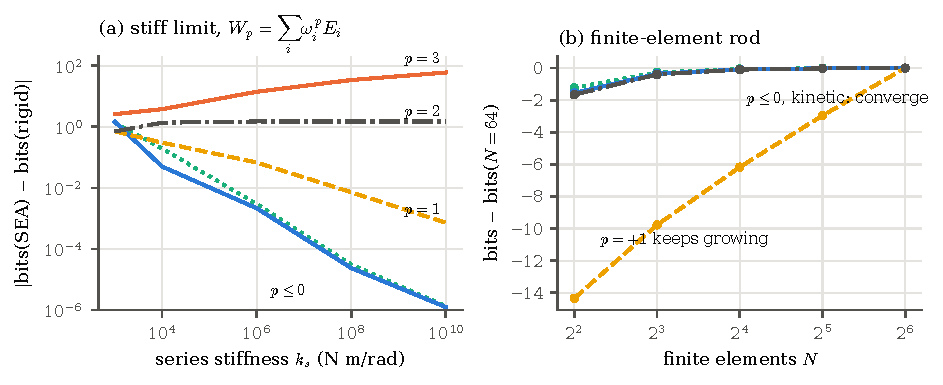
\includegraphics[width=\linewidth]{figures/alternatives.pdf}
\caption{(a) Stiff limit of the frequency-weighted metrics $W_p$: SEA minus rigid bits
against $k_s$. The gap vanishes for $p<2$, stalls at $p=2$ and diverges at $p=3$, as
predicted. (b) Mesh refinement of the rod, relative to $N=64$. Energy, action and the
kinetic metric converge; $p=+1$ does not (\code{check\_alternatives\_sea},
\code{check\_alternatives\_rod}).}
\label{fig:alternatives}
\end{figure}

\begin{proposition}[Data-driven whitening erases the body]\label{prop:datadriven}
Suppose the stacked response $y=Mw$ ($M$ of full column rank $d$) is whitened by its own
covariance, $(\sigma_w^2MM^\top)^{+1/2}$ on the range of $M$, and isotropic noise
$\sigma_n$ is then added. Then the information is $\frac d2\log_2(1+\sigma_n^{-2})$ for
\emph{every} body.
\end{proposition}
\begin{proof}
Write the thin SVD $\sigma_wM=U\Sigma V^\top$. The whitener is $U\Sigma^{-1}U^\top$, and
the whitened signal is $U\Sigma^{-1}U^\top U\Sigma V^\top(w/\sigma_w)=UV^\top(w/\sigma_w)$.
Its Gram matrix is $\sigma_n^{-2}VU^\top UV^\top=\sigma_n^{-2}I_d$. By \cref{lem:gauss},
the bits are $\frac12\log_2\det((1+\sigma_n^{-2})I_d)$.
\end{proof}

\phys{Whitening by the data, i.e.\ $z$-scoring or ZCA on the observed response, makes every
direction equally informative by construction, so the body's contribution vanishes. The
check gives 56.59 bits for the rigid leg and for SEAs at 70 and $10^4$, equal to the
prediction (\code{check\_data\_driven\_whitening}). The noise model must come from the body,
not from the data.}

%=========================================================================================
\section{A thermodynamically consistent body: Langevin noise}
\label{sec:langevin}

The paper's noise is added to the \emph{readout}, independently at each sample. A body
that is genuinely noisy is instead driven by thermal forces matched to its own dampers,
and its noise is then shaped by its dynamics. This section builds that model and asks
whether the paper's conclusions survive.

\paragraph{The model.} The equation of motion becomes
\[
  H\ddot q+D\dot q+Kq=J^\top f(t)+\xi(t),\qquad
  \E[\xi(t)\xi(s)^\top]=2\sigma_T^2D\,\delta(t-s),
\]
started from the Gibbs law $x_q(0)\sim\mathcal N(0,\sigma_T^2\Em^{-1})$ on the clamped
bench. By \cref{prop:fdt} the noise is stationary at covariance $P=\sigma_T^2\Em^{-1}$.
Sampling with step $\Delta t$ gives $x_{k+1}=A_dx_k+B_df_k+w_k$ with $w_k$ i.i.d.\
$\mathcal N(0,Q_d)$ and $Q_d=P-A_dPA_d^\top$; this is \code{gibbs\_pair}, scaled by
$\sigma_T^2$. We set $\sigma_T^2=\sigma^2=10^{-4}$\,J, so a snapshot of the noise has
exactly the covariance used in Part~I. Only its correlation over time differs.

\begin{proposition}[Full observation: an exact formula]\label{prop:innov}
If the full state is observed without readout noise, the information about the force
profile is
\[
  \bits=\tfrac12\log_2\det\!\big(I_d+\sigma_w^2\,g\,\bar\Phi^\top\bar\Phi\big),
  \qquad g=B_d^\top Q_d^{-1}B_d ,
\]
where $\bar\Phi$ holds the force basis at the samples that drive the state. The design
enters only through the scalar $g$, the per-sample signal-to-noise ratio of a unit force
against one thermal kick.
\end{proposition}
\begin{proof}
\emph{Step 1: change variables.} The map from $(x_0,x_1,\dots,x_N)$ to
$(x_0,e_0,\dots,e_{N-1})$, with $e_k=x_{k+1}-A_dx_k$, is invertible. So the two carry the
same information (\cref{lem:noise}a).

\emph{Step 2: what the new variables contain.} $x_0$ is independent of the force, and
$e_k=B_df_k+w_k$, where the $w_k$ are i.i.d., independent of $x_0$, and Gaussian with
covariance $Q_d$. This is a Gaussian channel with noise covariance $I\otimes Q_d$.

\emph{Step 3: apply the Gaussian formula.} Whiten the noise by $Q_d^{-1/2}$ and apply
\cref{lem:gauss} with $f_k=\sum_jw_j\bar\Phi_{kj}$. The Gram matrix is
$\sigma_w^2\sum_k\bar\Phi_k^\top(B_d^\top Q_d^{-1}B_d)\bar\Phi_k$, where $\bar\Phi_k$ is
row $k$ of $\bar\Phi$. Since $g$ is a scalar, this equals $\sigma_w^2g\,\bar\Phi^\top\bar\Phi$.
\end{proof}

\begin{proposition}[Only the dissipation at the contact matters]\label{prop:contact}
Suppose $J^\top$ lies in the range of $D$. As $\Delta t\to0$,
\[
  g\;\to\;\frac{\Delta t}{2\sigma_T^2}\,J D^+J^\top .
\]
With the full state observed, the information therefore depends only on $JD^+J^\top$: the
damping seen at the point where the force acts. For the paper's ground model, $JD^+J^\top=1/b_i$
for the rigid transmission and for every SEA, so every design gives the same bits.
\end{proposition}
\begin{proof}[Proof sketch]
\emph{Continuous time.} In the continuous-time limit, observing the state exactly is a
white-Gaussian-noise channel for the drift $Bf$, with noise intensity
$GG^\top=\diag(0,\,2\sigma_T^2H^{-1}DH^{-1})$. In the low-signal limit, where the causal
estimate of the signal is negligible, Duncan's theorem \citep{duncan1970calculation} gives
the information rate $\frac12\E[(Bf)^\top(GG^\top)^+(Bf)]$ nats per second.

\emph{The rate.} Substituting $B=[0;H^{-1}J^\top]$ gives
\[
  \tfrac12\E[f^2]\,JH^{-1}\big(2\sigma_T^2H^{-1}DH^{-1}\big)^+H^{-1}J^\top
  =\frac{\E[f^2]}{4\sigma_T^2}\,JD^+J^\top .
\]

\emph{Matching to the discrete channel.} Over one sample, the discrete channel carries
$\frac12\log(1+g\,\E[f^2])\approx\frac12g\,\E[f^2]$ nats about a force sample. The
continuous rate gives $\Delta t\,\E[f^2]\,JD^+J^\top/(4\sigma_T^2)$ over the same
interval. Equating the two gives the stated limit for $g$, which does not depend on the
signal amplitude.

\emph{The design-independence.}
\begin{itemize}[nosep]
  \item For the rigid leg, $D=b_ir^2$ and $J=-r$, so $JD^+J^\top=1/b_i$.
  \item For the SEA,
        $D=\left[\begin{smallmatrix}b_s+b_ir^2&-b_s\\-b_s&b_s\end{smallmatrix}\right]$ has
        $\det D=b_sb_ir^2$, so $(D^{-1})_{11}=b_s/(b_sb_ir^2)=1/(b_ir^2)$. With
        $J=(-r,0)$, this gives $JD^{-1}J^\top=1/b_i$, independently of $k_s$ and $b_s$.
\end{itemize}

\emph{What is not proved here.} We do not prove that the discrete position-block terms
leave the constant unchanged. The numbers below confirm it.
\end{proof}

\checked{
\begin{itemize}[nosep]
  \item $2\sigma_T^2 g/(\Delta t\,JD^+J^\top)$ is $1.0000$ at 4, 16 and 64\,kHz for the
        rigid leg and for SEAs at $k_s=70$, $10^4$ and $10^6$ (shown as $g\sigma_T^2
        f_s/JD^+J^\top=0.5000$ by \code{check\_langevin\_dt\_limit}). It deviates only for
        coarse sampling (0.19 at 100\,Hz).
  \item The exact formula of \cref{prop:innov} and a direct computation with the full
        stacked noise covariance agree, 37.74216 bits
        (\code{check\_langevin\_innovations}).
  \item At the paper's settings, \emph{every} design gives 37.742 bits with the full state
        observed.
\end{itemize}}

\phys{This is the thermal limit of force sensing. The force must be read against the
fluctuating force of the damper at the contact, whose strength is set by the
fluctuation--dissipation theorem (the mechanical analogue of Johnson--Nyquist noise \citep{nyquist1928thermal}). If the whole state is observed, the body's inertia and
stiffness are irrelevant: no morphology can beat the contact-damper limit.

The body's design matters only when the observation is \emph{partial}, which is always the
case for a real robot.}

\paragraph{Partial observation: what morphology does.} With noise injected through the
dampers, observing coordinates $C$ with readout noise $\varepsilon$ gives the Gram matrix
$\sigma_w^2M_C^\top(C\Sigma C^\top+\varepsilon^2I)^{-1}M_C$. Here $\Sigma$ is the stacked
noise covariance, with blocks $\Cov(x_k,x_l)=A_d^{k-l}P$ for $k\ge l$
(\code{langevin\_bits}). By data processing, observing a subset can never exceed the
full-state value. So 37.742 bits is a hard ceiling for every design and every sensor.

\begin{table}[t]\centering\small
\caption{Bits about the force profile ($B_w=100$\,Hz) under the Langevin body, for several
readouts, and under the readout-noise models of Part~I (\code{check\_langevin\_designs}).
Efficiency is motor bits divided by full-state bits.}
\label{tab:langevin}
\begin{tabular}{lrrrrrr}
\toprule
& \multicolumn{4}{c}{Langevin body} & \multicolumn{2}{c}{readout noise only}\\
\cmidrule(lr){2-5}\cmidrule(lr){6-7}
Design & full state & motor & efficiency & motor + encoder & energy & motor\\
\midrule
rigid            & 37.742 & 37.695 & 0.999 & 35.707 & 71.723 & 66.836\\
SEA $k_s=70$     & 37.742 &  2.266 & 0.060 &  1.637 & 69.280 & 24.379\\
SEA $10^3$       & 37.742 & 18.628 & 0.494 & 17.925 & 70.267 & 65.892\\
SEA $3\times10^3$& 37.742 & 29.038 & 0.769 & 28.194 & 71.084 & 72.780\\
SEA $10^4$       & 37.742 & 35.067 & 0.929 & 33.820 & 71.773 & 69.414\\
SEA $10^5$       & 37.742 & 37.242 & 0.987 & 35.631 & 71.742 & 67.104\\
SEA $10^6$       & 37.742 & 37.537 & 0.995 & 35.704 & 71.725 & 66.863\\
\bottomrule
\end{tabular}
\end{table}

Three findings (\cref{tab:langevin,fig:langevin}):
\begin{enumerate}
  \item \emph{The rigid transmission routes almost everything to its motor encoder.}
        Through the motor angle alone it captures 99.9\% of the thermal ceiling. The SEA's
        efficiency rises monotonically with stiffness: 6\% at the prototype's $k_s=70$,
        49\% at $10^3$, 93\% at $10^4$, 99.5\% at $10^6$. This is Wensing's argument for
        proprioceptive actuation, derived from first principles: the rigid transmission
        delivers contact information to the actuator's own sensor without loss.
  \item \emph{The readout-noise model can rank designs wrongly.} With fixed encoder noise
        added to the readout, the SEA at $k_s=3\times10^3$ beats the rigid leg by 5.9 bits
        through the motor encoder, and at $10^4$ by 2.6 bits. Under Langevin noise this cannot
        happen: the rigid leg is already within 0.05 bits of the ceiling, so no design can
        beat it by more.

        The difference is resonance. A passive resonance amplifies the force signal at the
        motor, and with readout-only noise that amplification looks like free SNR. Under
        fluctuation--dissipation the same resonance amplifies the thermal force noise by
        exactly the same factor, so it gains nothing. This is the duplicate-readout
        artifact again, now in the frequency domain.
  \item \emph{With full-state readout, the two models agree qualitatively.} Langevin noise
        plus energy readout noise gives 36.2--36.4 bits for every design. The
        energy-whitened readout model of Part~I gives 69.3--71.8. Both say the full state
        hardly separates the designs, whereas the motor encoder separates them strongly.
\end{enumerate}

\begin{figure}[t]\centering
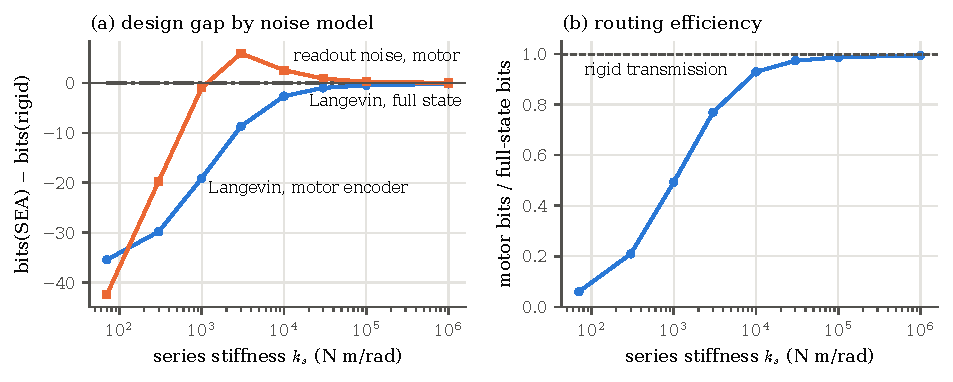
\includegraphics[width=\linewidth]{figures/langevin.pdf}
\caption{(a) SEA minus rigid bits through different noise models. Langevin noise with the
full state observed gives zero, to within $10^{-5}$ bits, for every design. Through the motor encoder,
Langevin noise gives a monotone climb to the rigid leg, while readout-only noise lets the
SEA overtake the rigid leg near $3\times10^3$. (b) Routing efficiency under Langevin noise:
the fraction of the thermal ceiling that reaches the motor encoder.}
\label{fig:langevin}
\end{figure}

\paragraph{Caveats.}
\begin{itemize}[nosep]
  \item $\sigma_T^2$ is an effective temperature, chosen to match Part~I.
  \item The ground damping $b_i$ is a modeling choice ($\zeta_{\rm contact}=0.15$),
        identical across designs by construction
        (\code{test\_one\_ground\_for\_every\_design}). The common ceiling is therefore a
        property of the ground model.
  \item Damping is modeled as constant and viscous. The model needs a positive-definite
        $\Em$, so it applies to the clamped bench only.
\end{itemize}

%=========================================================================================
\section{What energy whitening does and does not capture}
\label{sec:capture}

\begin{enumerate}
  \item \emph{Retention is settled.} For the question ``how much does the body itself hold
        about the world,'' energy is the unique admissible resolution
        (\cref{thm:unique}). Every information quantity built on it is coordinate-free,
        composes across components, converges in constraint and refinement limits, and
        changes only through work and dissipation (\cref{prop:work}).
  \item \emph{Routing is what morphology does.} In a thermodynamically consistent body the
        total is capped by the dissipation at the contact (\cref{prop:contact}). What
        distinguishes designs is how much of that total reaches the coordinates a
        controller can read, at a latency it can use. The efficiency of
        \cref{tab:langevin} is a candidate scalar measure of mechanical intelligence in
        this sense. The temporal and frequency decompositions of Part~I can be applied to
        it unchanged.
  \item \emph{Relevance is not captured.} Neither retention nor routing asks whether the
        information is about what the task needs. The paper's $I(W;X\mid A)$ measures
        relevance to the action. Task-specific variables, such as the force component that
        matters for balance, would sharpen this.
  \item \emph{Nonlinear and multistable bodies.} The framework extends directly: the noise
        law becomes the Gibbs law $\exp(-V/T)$ on a non-quadratic potential. A mechanical
        memory then stores a reliable bit when its energy barrier is large compared with
        the noise energy, the classical criterion behind Landauer's bound
        \citep{landauer1961irreversibility}. This connects the analysis to mechanical
        metamaterials and latching mechanisms, but none of it is tested here.
  \item \emph{Validation must be predictive.} A definition is checked by its consequences.
        The consistency checks pass: invariance, limits, Wensing's conclusions. The
        empirical test is whether retention, routing or relevance best predicts
        closed-loop performance across designs. The paper's Table~I hints at this.
\end{enumerate}

%=========================================================================================
\section{Limitations and open questions}
\label{sec:limits}
\begin{enumerate}
  \item \emph{Body versus sensor.} The energy noise model quantifies what the
        \emph{body} retains. Real encoders have per-coordinate noise, and the code's
        \code{"motor"} readout answers that different question. The two should be
        reported as distinct quantities; \cref{sec:langevin} shows how to combine them
        consistently.
  \item \emph{The environment lives in the metric.} $K$ includes the ground spring, so
        $\Em$ differs between stance and flight, and the ground stiffness can flip the
        sign of the SEA--rigid comparison
        (\code{test\_the\_ground\_decides\_whether\_series\_compliance\_helps\_or\_hurts}).
        This is physically right, since the ground does store energy, but it should be
        stated.
  \item \emph{Dissipation is not stored energy.} $D$ is absent from $\Em$, as it should
        be. Materials with internal variables (viscoelastic Maxwell elements) add states
        whose stored energy has to be defined first.
  \item \emph{Nonlinearity and contact.} $H(q)$ varies, contact switches $K$, and gravity
        preloads the stiffness. Remark~\ref{rem:scope} outlines a trajectory-wise
        extension. Hybrid contact needs a metric per mode and a rule at impacts.
  \item \emph{The noise scale.} $\sigma$ is a resolution, not a temperature. Comparisons
        are $\sigma$-robust only at equal excited rank (\cref{prop:snr}c), so ranks should
        be reported alongside bits.
  \item \emph{Two metrics, two questions.} $I(W;X)$ and $\mathrm{MC}_W$ measure
        transmission and retention respectively (\cref{prop:mcw}). They should not be
        expected to agree.
\end{enumerate}

%=========================================================================================
\section{How to proceed: decisions for discussion}
\label{sec:proceed}

Each item states a decision, the options, and a recommendation with its reason.

\begin{enumerate}
  \item \emph{How to justify the metric in the paper.} Options:
        \begin{itemize}[nosep]
          \item keep ``resembles approaches in [21]--[25]'';
          \item replace it with the uniqueness theorem (\cref{thm:unique}) and the
                information-preservation property (\cref{prop:work}), citing Jaynes for
                the shape.
        \end{itemize}
        \emph{Recommendation:} the second. It is a stronger, self-contained claim, and it
        removes reliance on citations that we could verify only through secondary
        sources.
  \item \emph{What to report.} Options: retained bits only (as now), or retained and
        routed bits side by side (body vs motor encoder).
        \emph{Recommendation:} side by side. The gap between them is where morphology does
        its work, and it is what reproduces Wensing's argument.
  \item \emph{Which noise model.} Options: keep readout noise and add the Langevin body as
        a robustness check, or make the Langevin body the main model.
        \emph{Recommendation:} keep readout noise for the full-state analyses of
        Sections~III--IV, where the two agree qualitatively. Use the Langevin body for
        anything that involves a sensor, since readout-only noise misranks resonant
        designs there (\cref{tab:langevin}).
  \item \emph{Predictive validation.} For the Go2 designs of Table~I, compute retention,
        routing efficiency and $I(W;X\mid A)$, and test which best predicts tracking
        error across designs and seeds. This is the empirical test the definitions
        currently lack.
  \item \emph{The simulated leg.} Repeat the Langevin comparison in MuJoCo by injecting
        damping-matched noise forces, and estimate with InfoNCE as in Sec.~IV. The
        prediction is that the full-state bits are flat across designs and the motor bits
        climb with stiffness.
  \item \emph{Floating base.} Decide how Sec.~V treats zero-energy base positions:
        velocities only, the $\omega_{\rm ref}^2H$ regularizer with a sensitivity sweep,
        or gravity and contact stiffness at the operating point (\cref{sec:floating}).
        The Langevin body also needs $\Em\succ0$ for its initial law, so this decision
        affects both models.
  \item \emph{Nonlinear and multistable extension.} Replace the quadratic energy by the
        actual potential, with noise law $\exp(-V/T)$. This is the natural route to
        mechanical memory and logic, and a possible follow-up paper rather than a
        revision item.
\end{enumerate}

%=========================================================================================
\appendix
\section{Suggested text for a revision}
\label{app:text}

\paragraph{Replacement for the whitening paragraph (Sec.~III-A).}
\begin{quote}\small
Because the response is deterministic, information is finite only once a resolution is
declared, and the result depends on the declaration alone. We declare it in energy: the
state is known up to Gaussian noise of covariance $\sigma^2\Em^{-1}$, with
$\Em=\diag(K,H)$. This is the maximum-entropy noise law at fixed mean energy
\citep{jaynes1957information}, i.e.\ the equilibrium-fluctuation shape at effective
temperature $\sigma^2$ \citep{kubo1966fluctuation}.

Equivalently, we observe the whitened state $x=\Em^{1/2}x_q$, in units of
$\sqrt{\mathrm J}$, with isotropic noise. The resulting information is exactly invariant
under any linear change of generalized coordinates or units. In the stiff limit it
converges to that of the corresponding rigid mechanism, whereas a per-coordinate noise
budget counts redundant coordinates as independent observations (8.47 bits here). In these
coordinates the dynamics take port-Hamiltonian form \citep{vanderschaft2014port}, and the
velocity block is the mass weighting of modal kinetic-energy sensor-placement methods
\citep{li2007connection}.

The energy metric is moreover the only noise metric that is coordinate-free, assembled
element by element without outside scales, symmetric in time, and invariant under the
body's free motion. The last property means that free motion can never create
information: under this metric the body gains information only through work done by the
environment and loses it only through dissipation.
\end{quote}

\paragraph{For the Shapley paragraph (Eq.~(10)).}
\begin{quote}\small
The noise is attached to the body, not to individual coordinates: observing a subset $S$
means observing those coordinates of the noisy state, with noise covariance
$\sigma^2(\Em^{-1})_{SS}$. The game is then monotone, and the full set recovers the total.
\end{quote}

\paragraph{For the Fig.~2 discussion.}
\begin{quote}\small
At high stiffness the joint and motor \emph{angles} become redundant, because their noise
becomes perfectly correlated, and receive equal Shapley credit. The two \emph{velocities}
remain independent observations whose precisions, $m_lr^2$ and $I_{\rm rot}$, sum to the
rigid inertia, so their credit is split in proportion to inertia.
\end{quote}

\section{Status of the literature claims}
\label{app:sources}

Full-text access was partly blocked from the analysis environment. The table records
exactly what each citation in this note rests on.
\begin{itemize}[nosep]
  \item \textbf{Full text}: read in the primary source; equation and section numbers are
        given only for these.
  \item \textbf{Secondary}: from abstracts or citing works.
\end{itemize}
Every mathematical statement in this note is proved here and does not rely on any
citation.

\begin{center}\small
\begin{tabular}{>{\raggedright}p{0.30\linewidth}p{0.13\linewidth}>{\raggedright\arraybackslash}p{0.47\linewidth}}
\toprule
Source & Access & What is used \\
\midrule
\citet{jaynes1957information} (paper [25]) & full text & Eqs.\ (2-4), (2-10); Sec.~3 (Boltzmann); footnote 6 (discrete only)\\
\citet{kessy2018optimal} & full text & Eq.~(4) rotational freedom; Eq.~(8) ZCA; Eqs.~(13)--(14) optimality\\
\citet{diggavi2001worst} & full text & Lemma II.2 (Ihara): Gaussian noise is worst at fixed covariance\\
\citet{vanderschaft2014port} & full text & Eq.~(4.10), input--state--output pH form\\
\citet{buithanh2013computational} & full text & Sec.~3.3, mass-weighted inner product\\
\citet{cotter2013mcmc} & full text & robustness under mesh refinement (abstract and Sec.~1)\\
\citet{kubo1966fluctuation} (paper [23]) & secondary & FDT links noise intensity to dissipation; equipartition\\
\citet{moore1981principal} (paper [22]) & secondary & Gramians, coordinate dependence, balancing\\
\citet{li2007connection} (paper [21]) & secondary & EfI--MKE connection via iteration and re-orthonormalization\\
\citet{lee2020geometric} (paper [24]) & secondary & affine-invariant metric on inertial parameters (parameter space, not state space)\\
\citet{zahedi2013quantifying} (paper [10]) & secondary & discrete $\mathrm{MC}_W=I(W';W\mid A)$, empirical distributions\\
\citet{wensing2017proprioceptive} (paper [7]) & secondary & model parameters, as reproduced in the paper's Sec.~III\\
\citet{cover2006elements} & secondary & Ch.~12 maximum entropy; colored-noise channels\\
\citet{kammer1991sensor}, \citet{papadimitriou2004optimal} & secondary & EfI as D-optimal design; entropy-based placement\\
\citet{willems1972dissipative}, \citet{stuart2010inverse} & secondary & storage functions; function-space viewpoint\\
\citet{dupont1973l2,baker1976error,geveci1984convergence} & secondary & semi-discrete FE convergence (an assumption of \cref{thm:mesh})\\
\citet{landauer1961irreversibility}, \citet{bennett1982thermodynamics} & secondary & reversibility of conservative dynamics; dissipation as erasure\\
\citet{callen1951irreversibility} & secondary & quantum FDT, $\frac{\hbar\omega}{2}\coth\frac{\hbar\omega}{2k_BT}$\\
\citet{nyquist1928thermal} & secondary & thermal noise set by dissipation\\
\citet{duncan1970calculation} & secondary & mutual information for signals in white Gaussian noise\\
\bottomrule
\end{tabular}
\end{center}

\section{Reproducing every number}
\label{app:repro}
\begin{itemize}[nosep]
\item \code{uv run python docs/whitening/checks.py} prints every quantity quoted here.
\item \code{uv run python docs/whitening/make\_figures.py} redraws every figure.
\item \code{uv run pytest tests/test\_energy\_whitening.py} asserts each theorem's numerical
  consequence. It runs in a few seconds, and no library code or golden table is changed.
\end{itemize}

\bibliographystyle{plainnat}
\bibliography{refs}
\end{document}
